%------------------------------------------------------------------------------
% IPOL LaTeX style guide and Example
% by rafael grompone von gioi, nicolas limare, jose-luis lisani and others
%------------------------------------------------------------------------------

% IPOL class is based on the standard LaTeX article class is used
% essentially in the same way. The layout must not be changed. Special
% IPOL commands are used to set the title, authors and abstract.

\documentclass{ipol}

% Do not use math notations and greek letters in the title.
\ipolSetTitle{DCT denoising}

% Author names must be separated with commas (,), not "and" or "&".
\ipolSetAuthors{First Author \ipolAuthorMark{1},
                Second Author\ipolAuthorMark{2}}

% Affiliations must contain the department, institution and country.
% Use a professional email address (no gmail, yahoo, etc).
% Do not add postal address.
\ipolSetAffiliations{%
\ipolAuthorMark{1} Department, Institution, Country
                   (\texttt{user@server.net})\\
\ipolAuthorMark{2} Department, Institution, Country
                   (\texttt{username@mailserver.edu})}

%------------------------------------------------------------------------------

% The link hereafter points to IPOL documentation for convenience
% in this document but must be replaced in your manuscript.
% The preprint link will not be known before the first preprint page
% is created. For early preprint versions, just don't use this command
% and the link will be set to the IPOL journal DOI address.
\ipolPreprintLink{http://www.ipol.im/}

%------------------------------------------------------------------------------

% Add packages and definitions here.
% Keep the package list as small as possible and include the package
% sources (packagename.sty) with your article source.
% These packages are loaded by the IPOL class or considered standard,
% and need not be provided with their source if they are used:
%   color, hyperref, graphicx, rotating
%   amsmath, amssymb, amsthm
% For algorithms, please use the algorithm2e package instead of
% algorithmx for simplicity and a uniform style.

% times new roman font
%\usepackage{mathptmx}


\usepackage[vlined,ruled]{algorithm2e}
% define input and output keywords
\SetKwInOut{Input}{input}
\SetKwInOut{Output}{output}
% define comment style
\SetKwComment{Comment}{}{}
\newcommand{\mycmtsty}[1]{\em \small #1}
\SetCommentSty{mycmtsty}

% Use \newtheorem{} for remarks and definitions.
\usepackage{amsthm}
\newtheorem{definition}{Definition}
\newtheorem*{remark}{Remark}

\usepackage{amsmath}
\usepackage{amsfonts}
\usepackage{amssymb}


\newcommand{\ma}[1]{\boldsymbol{#1}}

\DeclareMathOperator*{\argmin}{arg\,min}
\DeclareMathOperator*{\argmax}{arg\,max}


%------------------------------------------------------------------------------

\usepackage{fancyvrb}
\VerbatimFootnotes % allows verbatim text in footnotes

\begin{document}

% IPOL encourages authors to do joint submissions to IPOL and
% SIIMS (SIAM Journal of Imaging Science). Upon acceptance, cross
% references are placed between both articles. The environment
% ipolSIIMS is used to set the standard header, before the
% abstract. Uncoment these lines if you prepare an IPOL+SIIMS article:

%\begin{ipolSIIMS}
%This IPOL article is related to a companion publication in the SIAM
%Journal on Imaging Sciences:\\
%Author Names, ``Article Title.''
%\textsl{SIAM Journal on Imaging Sciences}, vol.~X, no.~X,
%pp.~N--M, YYYY. \url{http://dx.doi.org/10.1137/XXXXXXXXX}
%\end{ipolSIIMS}

%------------------------------------------------------------------------------
% The abstract of an IPOL article must be informative and summarize all
% important parts of the article. 

\begin{ipolAbstract}
Study of several variants of the DCT denoising algorithm. Some of them attain the quality of Non-Local Bayes at a tenth of the cost. On line demo available at the address: \url{http://dev.ipol.im/~facciolo/ipol_demo/dct2step}.
\end{ipolAbstract}

%------------------------------------------------------------------------------
% Use the source code info to briefly explain what can be found as
% software code in the IPOL article.
% Do not use the phrasing "...the IPOL web part of this article."

\begin{ipolCode}
The source code section briefly explains what the source code
published with the article contains, all in a single paragraph. For
example: The reviewed source code and documentation for this algorithm
are available from \href{\ipolLink}{the web page of this
  article}. Compilation and usage instruction are included in the
\verb|README.txt| file of the archive.
\end{ipolCode}


%------------------------------------------------------------------------------
% Use the supplementary files info to add explanations about other
% files published with the article.

\begin{ipolSupp}
The supplementary files section provides explanations about other
files published with the article, all in a single paragraph. Mention
clearly if they are reviewed or not. For example: A reference dataset,
to be used for further comparisons, is provided with the article and
peer-reviewed. A Matlab interface (not reviewed) is also available for
convenience.
\end{ipolSupp}

%------------------------------------------------------------------------------
% All papers need key words. Key words are lowercase except for proper
% names and acronyms, and separated with commas. Only use plain text.

\ipolKeywords{first, second, third, fourth}

%------------------------------------------------------------------------------
% Article content starts here.


%%%%%%%%%%%%%%%%%%%%%%%%%%%%%%%%
\section{Basic 2 step DCT denoising}
The simplest DCT denosing algorithm as described by Yu and Sapiro in \cite{dct2011} consists in a threshold of a patch-wise DCT of the image and aggregation of the resulting patches. Color images are first pre-processed with to de-correlate the input colors. Algorithm \ref{alg:dct} summarized it. Unlike the implementation of Yu and Sapiro the algorithm below  only uses a small amount of memory to process the image, as the extraction and processing of each patch is performed in a single loop, which can also be parallelized. Moreover, using the FFTW library to compute the DCT transforms further accelerates the processing. 

Let us note that although thresholding the DCT of a single patch introduces ringing artifacts, the patch-wise aggregation limits them in the final result. 

A guide image is a clean but not completely restored result, which could be used to determine the power spectrum of underlying signal. Algorithm \ref{alg:dct2} shows how to use a guide image as an oracle for a Wiener filter.
The two-step DCT denoising is then summarized in algorithm \ref{alg:2stepdct}. 


%%%%%%%%%%%%%%%%%%%%%%%%%%%%%%%%
\section{Iterated DCT denoising}

Following the previous argument one should continue applying the Wiener step on using the previous result as guide (as in algorithm \ref{alg:iterated}). In table \ref{tab:compare} we see a consistent improvement with respect to the basic 2-step result. 
In figures \ref{fig:res4}, \ref{fig:res8}, and \ref{fig:res16} we can compare the results obtained with different windows sizes.
In general the results get sharper with iterations, but in the process some artifacts are also amplified.


\begin{algorithm}
\DontPrintSemicolon
\Input{Noisy image $Y$, noise level $\sigma$, block size $s$}
\Output{Denoised image $X$}

$G \gets  \text{DCTdenoisingHard}(Y,\sigma, s)$\;

$X \gets  \text{DCTdenoisingWiener}(Y,G,\sigma, s)$\;

\caption{two-step DCT Denoising}
\label{alg:2stepdct}

\end{algorithm}







\begin{algorithm}
\DontPrintSemicolon
\Input{Noisy image $Y$, noise level $\sigma$, block size $s$}
\Output{Denoised image $X$}

$G \gets  \text{DCTdenoisingHard}(Y,\sigma, s)$\;

\For{$iter \gets 1 \ldots 10$ } {
$X \gets  \text{DCTdenoisingWiener}(Y,G,\sigma, s)$\;
$G \gets X$\;
}
\caption{Iterated DCT Denoising}
\label{alg:iterated}

\end{algorithm}






\begin{algorithm}
\DontPrintSemicolon
\Input{Noisy image $Y$, noise level $\sigma$, block size $s$}
\Output{Denoised image $X$}

$X, W \gets  0$\;

$Y \gets   \text{DecorrelateColors}(Y)$\;
\For{$patch \in \Omega$}{
	$ \widehat{b} \gets  \text{DCT}(\text{ExtractPatch}(Y, patch, s))$\;
    \For{$\omega \in supp(\widehat{b})$}{
    	
    	\If{$|\widehat{b}(\omega)|^2 < 3\sigma^2$}{
        	$\widehat{b}(\omega) \gets  0$\;
        }
    }
	$ {b} \gets  \text{IDCT}(\widehat{b})$\;
    $X(\Omega_{patch}) \gets  b $\;
    $W(\Omega_{patch}) \gets  W(\Omega_{patch}) +1 $\;
    
}

    $ X \gets  X / W$ \;
	$X \gets   \text{UndoDecorrelateColors}(X)$\;

\caption{DCT Denoising - Hard thresholding}

\label{alg:dct}

\end{algorithm}



\begin{algorithm}
\DontPrintSemicolon
\Input{Noisy image $Y$, guide $G$, noise level $\sigma$, block size $s$}
\Output{Denoised image $X$}

$X, W \gets  0$\;

$Y \gets  \text{DecorrelateColors}(Y)$\;
$G \gets  \text{DecorrelateColors}(G)$\;

\For{$patch \in \Omega$}{

	$ \widehat{b} \gets  \text{DCT}(\text{ExtractPatch}(Y, patch, s))$\;
  	$ \widehat{g} \gets  \text{DCT}(\text{ExtractPatch}(G, patch, s))$\;
    
    \For{$\omega \in supp(\widehat{b})$}{
    	$ \widehat{b}(\omega) \gets   \widehat{b}(\omega) \left({\displaystyle \frac{|\widehat{g}(\omega)|^2 }{|\widehat{g}(\omega)|^2 +\sigma^2}}\right)$
    }
	$ {b} \gets  \text{IDCT}(\widehat{b})$\;
    $X(\Omega_{patch}) \gets  b $\;
    $W(\Omega_{patch}) \gets  W(\Omega_{patch}) +1 $\;
    
}

    $ X \gets  X / W$ \;
	$X \gets  \text{UndoDecorrelateColors}(X)$\;

\caption{DCT Denoising - Wiener}

\label{alg:dct2}


\end{algorithm}

%%%%%%%%%%%%%%%%%%%%%%%%%%%%%%%%
\section{Multiscale DCT denoising}

The multiscale DCT denoising uses Nicola Pierazzo's multiscaler algorithm for cutting and recomposing the results computed at different scales \cite{multiscaler2016}. Both the causal and non-causal multiscale algorithms produce similar results (we show the causal). 
We observe in table \ref{tab:compare} that only for small patch sizes the result improves with respect to the 2-step single-scale DCT denoising. The results with multiscale shown in figures \ref{fig:res4}, \ref{fig:res8}, and \ref{fig:res16} are smoother than their single scales counterparts. 



%%%%%%%%%%%%%%%%%%%%%%%%%%%%%%%%
\section{Iterated, guided multiscale DCT denoising}

We tested the iterated multiscale algorithm described in algorithm \ref{alg:itermulti}. The iterations are applied on the complete non-causal multiscale algorithm, using the result of the previous iteration as guide. The results are reported in table \ref{tab:compare}.


\begin{algorithm}[h!]
\caption{Iterated guided multiscale DCT Denoising}
\label{alg:itermulti}
\Input{Noisy image $Y$,  noise level $\sigma$, block size $s$, and $n_{scales}$}
\Output{Denoised image $combined$}

     $G \gets \text{DCTdenoising2step}(Y,  \sigma, 8)$ \hfill  \tcc{Bootstrap iterations with a good guide (block\_sz=8)}

  \For{$iter \gets 1 \ldots 10$}{
  
  $combined \gets$ NULL \hfill \tcc{{Non-causal multiscale}}
  \For{$scale \gets n_{scales} - 1, \ldots, 0$}{
     $Y_s \gets\text{ExtractScale}(Y,  scale)$\;
     $G_s \gets\text{ExtractScale}(G,  scale)$\;
     $X_s \gets\text{DCTdenoisingWiener}(Y_s, G_s, \sigma, s)$\;

   $combined \gets \text{MergeCoarse}(X_s, combined)$\;

  }
  $G\gets combined $  \hfill \tcc{Update guide}
  }
  
\end{algorithm}


The best results are obtained with $4\times 4$ windows, improving on the results of multiscale DCT, and iterated DCT  by 0.1 dB.
Note that the best result of iterated DCT is obtained with windows of $16\times 16$ ( 16 times slower than $4\times 4$), thus algorithm \ref{alg:itermulti} is also cheaper. Figure \ref{fig:psnr_iter} shows the evolution of the PSNR with the iterations.
 
The results are noticeably sharper than the ones of DCT denoising but also have several small artifacts.





%%%%%%%%%%%%%%%%%%%%%%%%%%%%%%%%
\section{Postprocess with DA3D}

The DA3D post-process \cite{Pierazzo2015} uses a guide image to produce an improved denoised result. In the last section of table \ref{tab:compare} are compared the PSNRs of various  post-processed results obtained with DA3D, concretely including NL-Bayes \cite{Lebrun2013}, NL-Bayes Multiscale and several Multiscale DCT denoising. 

Note that the results obtained using DCT denoising guides improve substantially in terms of PSNR, the results are comparable to those of NL-Bayes. This is because da3d suppresses most of the artifacts of DCT denoising as seen in figure \ref{fig:da3d}. 
In particular the result of \emph{"dct4 multi4 + da3d"} exhibits very little residual ringing.

In terms of efficiency the difference is substantial. For the  1.3MP image shown in figure \ref{fig:da3d} the computation (on a 4-cores computer) of \emph{"dct4 multi4 + da3d"} takes 30 seconds, while \emph{"NL-Bayes multi3 + da3d"} takes 5 minutes 10 seconds (ten times slower!). 



\begin{figure}[htbp]
\begin{center}
\includegraphics[width = .9\textwidth]{f/graphPSNR_dct4_multi_iter} 
\caption{{\bf PSNR evolution} for iterated guided multiscale DCT denoising ($w=4$), starting from DCT 2-step ($w=8$).}
\label{fig:psnr_iter}
\end{center}
\end{figure}









\begin{table}%[h!]
\caption{Results obtained on the image \emph{Sans\_bruit\_1} with noise $\sigma =50$. }
\begin{center}
\begin{tabular}{l|c}
\bf Algo & \bf PSNR \\
\hline
NL-Bayes & 28.194\\
NL-Bayes multi3& 28.305\\

\hline
\hline

dct4 1step& 24.897 \\ 
dct4 2step& 25.312 \\
dct4 iter10& 25.505 \\
% ./dctdenoising_multiscale.sh  $n $s rr.tif "-w 4" 4; imgerr PSNR $o rr.tif;
dct4 multi4 &  27.747\\

\hline
dct8 1step& 26.917 \\ 
dct8 2step& 27.294 \\
dct8 iter10& 27.471 \\
dct8 multi4 &  27.779\\

\hline
dct16 1step& 27.329 \\
%./dctdenoising -w 16 $n $s rr.tif; imgerr PSNR $o rr.tif; iion rr.tif dct16_2step.png;     for i in `seq 1 10`; do ./dctdenoising -w 16 $n $s -2 rr.tif rr.tif; imgerr PSNR $o rr.tif; done; iion rr.tif dct16_iter10.png 
dct16 2step& 27.680 \\
dct16 iter10& 27.840 \\
dct16 multi4 &  27.483\\

\hline
\hline
dct4 multi4 iter10& 27.878 \\
dct8 multi4 iter10& 27.993 \\

\hline
\hline
NL-Bayes + da3d & 28.485\\
NL-Bayes multi3 + da3d & 28.624\\
dct4 multi4 + da3d &  28.374\\
dct8 multi4 + da3d &  28.355\\
dct16 multi4 + da3d &  28.206\\
dct4 multi4 iter10 + da3d& 28.503 \\
dct8 multi4 iter10 + da3d& 28.515 \\
\end{tabular}
\end{center}
\label{tab:compare}
\end{table}%







%%%%%%%%%%%%%%%%%%%%%%%%%


\begin{figure}[htbp]
\begin{center}
\begin{tabular}{cc}

\includegraphics[width = .44\textwidth]{f/dct4_1step} &
\includegraphics[width = .44\textwidth]{f/dct4_2step} \\
dct4 1step (24.897) & dct4 2step (25.312) \\
\includegraphics[width = .44\textwidth]{f/dct4_iter10} &
\includegraphics[width = .44\textwidth]{f/dct4_multi4} \\
dct4 iter10 (25.505) &  dct4 multi4 (27.747)\\


\end{tabular}
\caption{{\bf results} of algorithms \ref{alg:dct}, \ref{alg:2stepdct},  \ref{alg:iterated}, and Pierazzo's multiscale DCT \cite{multiscaler2016},  all using  $4 \times 4$ windows.}
\label{fig:res4}
\end{center}
\end{figure}



\begin{figure}[htbp]
\begin{center}
\begin{tabular}{cc}

\includegraphics[width = .44\textwidth]{f/dct8_1step} &
\includegraphics[width = .44\textwidth]{f/dct8_2step} \\
dct8 1step (26.917) & dct8 2step (27.294) \\
\includegraphics[width = .44\textwidth]{f/dct8_iter10} &
\includegraphics[width = .44\textwidth]{f/dct8_multi4} \\
dct8 iter10 (27.471) &  dct8 multi4 (27.779)\\


\end{tabular}
\caption{{\bf results} of algorithms \ref{alg:dct}, \ref{alg:2stepdct},  \ref{alg:iterated}, and Pierazzo's multiscale DCT \cite{multiscaler2016},  all using  $8 \times 8$ windows.}
\label{fig:res8}
\end{center}
\end{figure}



\begin{figure}[htbp]
\begin{center}
\begin{tabular}{cc}

\includegraphics[width = .44\textwidth]{f/dct16_1step} &
\includegraphics[width = .44\textwidth]{f/dct16_2step} \\
dct16 1step (27.329) & dct16 2step (27.680) \\
\includegraphics[width = .44\textwidth]{f/dct16_iter10} &
\includegraphics[width = .44\textwidth]{f/dct16_multi4} \\
dct16 iter10 (27.840) &  dct16 multi4 (27.483)\\


\end{tabular}
\caption{{\bf results} of algorithms \ref{alg:dct}, \ref{alg:2stepdct},  \ref{alg:iterated}, and Pierazzo's multiscale DCT \cite{multiscaler2016},  all using  $16 \times 16$ windows.}
\label{fig:res16}
\end{center}
\end{figure}

%%%%%%%%%%%%%%%%%%%%%%
\begin{figure}[htbp]
\begin{center}
\begin{tabular}{cc}

\includegraphics[width = .44\textwidth]{f/orig} &
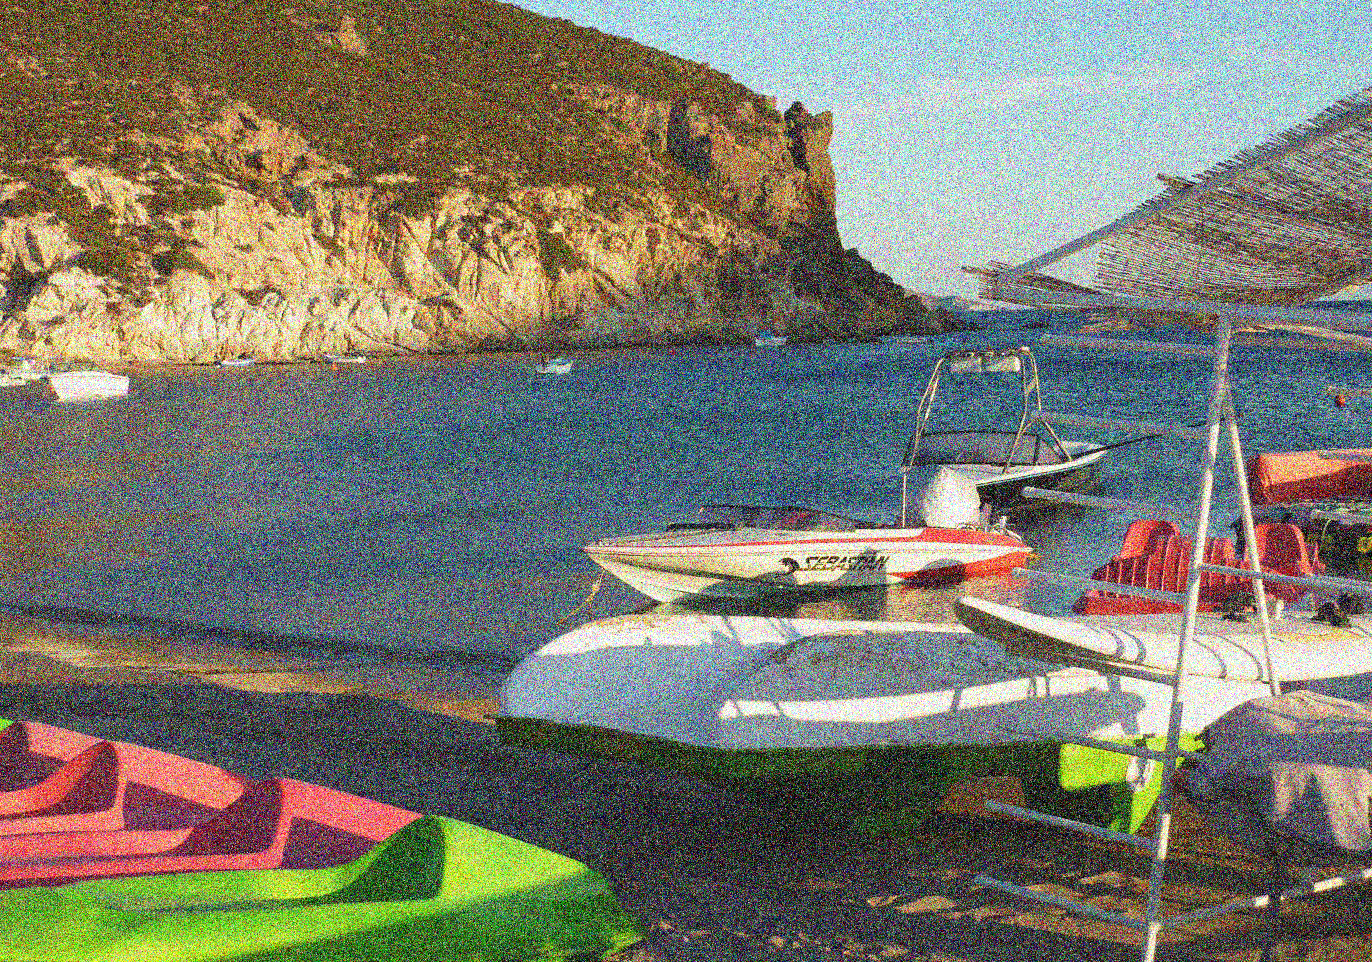
\includegraphics[width = .44\textwidth]{f/noisy} \\
original noiseless  & nosiy ($\sigma=50$) \\

\includegraphics[width = .44\textwidth]{f/nlb} &
\includegraphics[width = .44\textwidth]{f/nlb_multi3} \\
 NL-Bayes (28.194) &  NL-Bayes multi3 (28.305)  \\

\includegraphics[width = .44\textwidth]{f/dct4_multi4_iter10}&
\includegraphics[width = .44\textwidth]{f/dct8_multi4_iter10}\\
dct4 multi4 iter10 (27.878) &  dct8 multi4 iter10 (27.993) \\

\end{tabular}
\caption{{\bf results} of NL-Bayes \cite{multiscaler2016} and algorithm \ref{alg:itermulti} for two window sizes}
\label{fig:itermulti}
\end{center}
\end{figure}


%%%%%%%%%%%%%%%%%%%%%%
\begin{figure}[htbp]
\begin{center}
\begin{tabular}{cc}

\includegraphics[width = .44\textwidth]{f/nlb_da3d} &
\includegraphics[width = .44\textwidth]{f/nlb_multi3_da3d} \\
NL-Bayes+ da3d (28.485)    & NL-Bayes multi3 + da3d (28.624)  \\

\includegraphics[width = .44\textwidth]{f/dct4_multi4_da3d} &
\includegraphics[width = .44\textwidth]{f/dct8_multi4_da3d} \\
dct4 multi4 + da3d (28.374) &  dct8 multi4 + da3d (28.355)  \\

\includegraphics[width = .44\textwidth]{f/dct4_multi4_iter10_da3d}&
\includegraphics[width = .44\textwidth]{f/dct8_multi4_iter10_da3d}\\
dct4 multi4 iter10 + da3d (28.503) &  dct8 multi4 iter10  + da3d (28.515) \\

\end{tabular}
\caption{{\bf results} post-processed with DA3D \cite{Pierazzo2015}.}
\label{fig:da3d}
\end{center}
\end{figure}





\newpage

\section{RAW results and script calls (don't look, incorrect PSNRs)}

Using Dice, with noise $\sigma=40$

\begin{enumerate}
\item NLB single scale: 36.4 dB
\item NLB multiscale: 35.25 dB
\item DCT denoising Wiener-step using GT as guide (w=16/w=8): 36.49/34.55 dB
\item DCT denoising 2-step (w=16/w=8): 34.06/31.73 dB
\item iterated DCT denoising 2-step, 10 iterations, using DCT 2-step as initial point, (w=16/w=8/w=4): 24.88/24.74/24.01 dB
\item  

\end{enumerate}




\begin{verbatim}

 1294  ./dctdenoising.ok ../diceN.tif -w 16 40 -2 ../dice.png ref16.tif; imgerr PSNR ../dice.png ref16.tif 
 1295  ./dctdenoising.ok ../diceN.tif -w 8 40 -2 ../dice.png ref8.tif; imgerr PSNR ../dice.png ref8.tif 

 1299  ./dctdenoising.ok ../diceN.tif -w 16 40 dct16.tif; imgerr PSNR ../dice.png dct16.tif 
 1300  ./dctdenoising.ok ../diceN.tif -w 8 40 dct8.tif; imgerr PSNR ../dice.png dct8.tif 
 
 1301  cp dct16.tif rr.tif; for i in `seq 1 10`; do  ./dctdenoising ../diceN.tif -w 16 40 -2  rr.tif rr.tif; imgerr PSNR ../dice.png rr.tif;   done; cp rr.tif rr16.tiff
 
 1302  cp dct8.tif rr.tif; for i in `seq 1 10`; do  ./dctdenoising ../diceN.tif -w 8 40 -2  rr.tif rr.tif; imgerr PSNR ../dice.png rr.tif;   done; cp rr.tif rr8.tiff
 
 
 1314  ./dctdenoising_multiscale.sh ../diceN.tif 40 /tmp/dm4.tif  "-w 4 " 4; imgerr PSNR ../dice.png /tmp/dm4.tif
 1316  ./dctdenoising_multiscale.sh ../diceN.tif 40 /tmp/dm8.tif  "-w 8 " 4; imgerr PSNR ../dice.png /tmp/dm8.tif
 1317  ./dctdenoising_multiscale.sh ../diceN.tif 40 /tmp/dm16.tif  "-w 16 " 4; imgerr PSNR ../dice.png /tmp/dm16.tif
 
 

w=4
s=50
../b/dctdenoising -w 8 $n $s rr.tif; 
for i in `seq 1 10`; do
	../multi/dctdenoising_multiscale_guided.sh $n rr.tif $s /tmp/t.tif "-w ${w}" 5; 
	imgerr PSNR /tmp/t.tif $o; 
	cp /tmp/t.tif rr.tif; 
done
cp rr.tif /tmp/xm_guided4_dct8.tif

\end{verbatim}




\section{Non-local DCT denoising} 

We explore in the following a non-local version of the block DCT denoising
algorithm. This approach is complementary to the multiscale approach and both 
could be combined together.

The idea of the non-local DCT algorithm is to group together similar patches.
This is mainly motivated by two reasons:
\begin{itemize}
	\item A group of similar patches could be centered before denoinsing using
		DCT shrinkage. With the center removed, we expect to alleviate the problem
		of ringing around contrasted image edges. A contrasted edge should dominate the
		patch distance and therefore would be present in all patches in the
		group. If the group's baricenter captures the edge, it will be removed from the
		centered patches. In practice, the patches in the group might be slightly shifted.
		The mean patch would then be a smoothed version of the edge, which means that
		the centered patches will have some high frequency components due to the edge residual.
	\item The group of similar patches provides more reliable estimates of the signal 
		statistics. This is useful for estimating the optimal shrinkage functions from the 
		patches in the group.
\end{itemize}

We focus on two-step approaches such as the ones outlined in Algorithms 
\ref{alg:2step_nldct}, \ref{alg:nldct1} and \ref{alg:nldct1}. Both steps
follow the same scheme. For each patch $p$, the $n$ nearest neighbors are 
searched for in a search window centered at $p$. The resulting group of
patches is filtered by a DCT shrinkage operator. The filtered patches are 
aggregated on the denoised image estimate. The second step uses the output
of the first step to determine the $n$ nearest neighbors and to guide the 
DCT shrinkage. In the following we will describe different options to use as
shrinkage operators.


\begin{algorithm}
\DontPrintSemicolon
\Input{Noisy image $Y$, noise level $\sigma$, block size $s$}
\Output{Denoised image $X$}
$G \gets  \text{NLDCT-Shrinkage}(Y,\sigma, s)$\;
$X \gets  \text{NLDCT-GuidedShrinkage}(Y,G,\sigma, s)$\;
\caption{Two-step NL-DCT Denoising}
\label{alg:2step_nldct}
\end{algorithm}

\begin{algorithm}
\DontPrintSemicolon
\Input{Noisy image $Y$, noise level $\sigma$, block size $s$, search radius $w$, number of NN $n$}
\Output{Denoised image $X$}
$X, W \gets  0$\;
$Y \gets   \text{DecorrelateColors}(Y)$\;
\For{$p \in \Omega$}{
	$\mathcal I \gets \text{SearchNearestNeighbors}(G,p,s,w,n)$\;
	$\mathcal P \gets \text{ExtractPatches}(Y,\mathcal I,s)$\;
	$\widehat{\mathcal P} \gets  \text{DCTGuidedShrinkGroup}(\mathcal P)$\;
	$X\gets \text{AggregatePatchesInGroup}(X, \mathcal I, \widehat{\mathcal P})$\;
	$W\gets \text{AggregateWeightsInGroup}(W, \mathcal I)$\;
}
$ X \gets  X / W$ \;
$X \gets   \text{UndoDecorrelateColors}(X)$\;
\caption{NL-DCT shrinkage}
\label{alg:nldct1}
\end{algorithm}

\begin{algorithm}
\DontPrintSemicolon
\Input{Noisy image $Y$, guide $G$, noise level $\sigma$, block size $s$, search radius $w$, number of NN $n$}
\Output{Denoised image $X$}
$X, W \gets  0$\;
$Y \gets   \text{DecorrelateColors}(Y)$\;
$G \gets   \text{DecorrelateColors}(G)$\;
\For{$p \in \Omega$}{
	$\mathcal I \gets \text{SearchNearestNeighbors}(G,p,s,w,n)$\;
	$\mathcal P \gets \text{ExtractPatches}(Y,\mathcal I,s)$\;
	$\mathcal G \gets \text{ExtractPatches}(G,\mathcal I,s)$\;
	$\widehat{\mathcal P} \gets  \text{DCTGuidedShrinkGroup}(\mathcal P,\mathcal G)$\;
	$X\gets \text{AggregatePatchesInGroup}(X, \mathcal I, \widehat{\mathcal P})$\;
	$W\gets \text{AggregateWeightsInGroup}(W, \mathcal I)$\;
}
$ X \gets  X / W$ \;
$X \gets   \text{UndoDecorrelateColors}(X)$\;
\caption{NL-DCT guided shrinkage}
\label{alg:nldct2}
\end{algorithm}

\subsection{Bayesian shrinkage operators for unitary transforms}

Most common shrinkage operators can be given a Bayesian interpretation with a
prior in the family of \emph{generalized Gaussian distributions}. This is often 
desirable since the Bayesian setting provides principled ways to set the parameters
given estimates of the signal statistics.
The following discussion was adapted from \cite{Moulin1999} and \cite{Elad2006shrinkage}.

We consider a signal $\ma p\in\mathbb R^d$ that we want to estimate from a
noisy observation $\ma q = \ma p + \ma n$, where $\ma n \sim \mathcal
N(0,\sigma I)$ is AWGN. In our setting the signal is typically a patch
extracted from a larger image. We will estimate $\ma p$ by assuming a suitable
prior distribution $\mathbb P(\ma p)$ and computing the MAP:
\[\hat{\ma p} = \argmin \frac1{2\sigma^2}\|\ma p - \ma q\|^2 - \ln \mathbb P(\ma p).\]

We consider priors in the following family of generalized Gaussian distributions:
\begin{equation}
	\mathbb P(\ma p\,|\,\bar{\ma p}, \Lambda, U, \nu) = 
	\left(\frac{\nu\eta(\nu)}{2\Gamma(1/\nu)}\right)^d\frac1{|\Lambda|^{1/2}}
	\exp\left(-\|\eta(\nu)\Lambda^{-1/2}U^T(\ma p - \bar{\ma p}) \|_{\nu}^\nu\right),
	\label{eeq:ggd-family}
\end{equation}
where $\Gamma$ is the gamma function, 
$U$ is an orthogonal matrix,
$\Lambda = \text{Diag}(\lambda_1,\lambda_2,\dots,\lambda_d)$ is a positive
definite diagonal matrix, $\|\,\cdot\,\|_\nu$ is the $\nu$-norm in $\mathbb
R^d$ for $\nu > 0$, 
$\eta(\nu) = \Gamma(3/\nu)^{1/2}\Gamma(1/\nu)^{-1/2}$
is a normalization factor, 
and $\bar{\ma p}$ is the mean of the distribution.  The
parameter $\nu$ is called the \emph{shape parameter}. With $\nu = 2$
recover the Gaussian distribution with covariance matrix $\Sigma = U\Lambda U^T$.
This allows us to interpret the $U$ as the orthonormal basis of principal
directions and $\lambda_i$ as analog to the variance along principal direction $\ma u_i$.

Decreasing the value of $\nu$ has the effect of 
increasing the tails and the probability of values close to the mean. When
$\nu \leqslant 1$, it can be shown that the resulting MAP favours sparse
solutions. A common choice in the wavelet denoising literature is to set $\nu = 1$, 
the \emph{Laplace distribution}. This follows from the observation that the
statistics of wavelet coefficients in natural images follows a GGD-like
distribution with shape parameter $\nu \leqslant 1$, and the Laplace
distribution is attractive for its computational simplicity.

This multivariate GGD can be factorized 
as the product of one dimensional GGDs along the principal directions.%
\footnote{There are other definitions of the multivariate GGD for which this
factorization does not hold. In particular, the multivariate GGD can be defined using the
$2$-norm instead of the $\nu$-norm. In this case, $\mathbb P(\ma
p\,|\,\bar{\ma p}, \Sigma,\nu) \propto \exp\left(-\frac12\|\Sigma^{-1/2}(\ma p
- \bar{\ma p}) \|_2^{2\nu}\right)$. When $\nu = 2$ the Gaussian distribution is recovered. Except in this case,
this PDF cannot be written as a product of 1D GGD. 
This definition maintains the level sets of the Gaussian distribution: ellipses
centered at $\bar{\ma p}$.  The definition given above with the $\nu$-norm
given above is anisotropic and depends on the choice of the
coordinate system.}
Define the principal components as $\ma \alpha = U^T(\ma p - \bar{\ma p})$. Then
\begin{equation}
	\mathbb P(\ma p\,|\,\bar{\ma p}, \Lambda, U, \nu) = \prod_{i =1}^d
	\frac{\nu\eta(\nu)}{2\Gamma(1/\nu)}\frac1{\lambda_i^{1/2}}
	\exp\left(-\left(\frac{\eta(\nu)|\alpha_i - \bar{\alpha}_i|}{\lambda_i^{1/2}}\right)^{\nu} \right).
	\label{eeq:ggd-family-factorized}
\end{equation}
Each principal component is therefore independent from the others. 

\subsubsection{Inference}

The independent of components
greatly simplifies the computation of the MAP, which is decomposed into $d$
one-dimensional optimization problems%
\footnote{Note that the MAP is separable only if the noise PDF is a function of
the 2-norm $\|\ma p - \ma q\|$.}.
Indeed, since $\|\ma p - \ma q\| = \|\ma \alpha - \ma \beta\|$, for $\ma \beta =
U^T\ma q$, we can express the MAP as follows
\[\hat{\ma \alpha} = \argmin \sum_{i = 1}^d\frac1{2\sigma^2} (\alpha_i -
\beta_i)^2 + \frac{\nu(\eta)^{\nu}}{\lambda_i^{\nu/2}}{|\alpha_i - \bar{\alpha}_i|^\nu}.\]

Let us now focus on the solution of the $i$-th principal component. We will
redefine $\ma \alpha$ and $\ma \beta$ as the centered variables $\ma \alpha -
\bar{\ma \alpha}$ and $\ma \beta - \bar{\ma \alpha}$. Then we have
\[\hat \alpha_i = \argmin \frac1{2\sigma^2} (\alpha_i -
\beta_i)^2 + \frac{\nu(\eta)^{\nu}}{\lambda_i^{\nu/2}}{|\alpha_i - \bar{\alpha}_i|^\nu}.\]
If $\nu \leqslant 1$ this function is non-differentiable at $\alpha_i = 0$.
The minimizer can be located in $\alpha_i = 0$ or in the zeros of its derivative: 
\[\beta_i = \alpha_i + \frac{\nu\eta(\nu)^{\nu}\sigma^2}{\lambda_i^{\nu/2}}|\alpha_i|^{\nu-1}.\]

We will distinguish three cases: $\nu = 2$, $\nu = 1$ and $\nu \to 0$. The case $\nu = 2$
corresponds to the Wiener filter. When $\nu = 1$, we can express the solution
with a soft-thresholding operator:
\[\hat\alpha_i = \left\{
\begin{array}{l l}
	0,& \displaystyle\text{if }|\beta_i| < \sqrt{2} \sigma^2{\lambda_i^{-1/2}},\\
	\displaystyle\beta_i - \sqrt{2} \sigma^2{\lambda_i^{-1/2}}\text{sign}(\beta_i),&\text{else.}
\end{array}
\right.\]

When $\nu\to 0$, \cite{Moulin1999} showed that the solution converges can be
obtained as the following hard-thresholding operator:
\[\hat\alpha_i = \left\{
\begin{array}{l l}
	0,& \displaystyle\text{if }|\beta_i| < \tau_\nu,\\
	\displaystyle\beta_i,&\text{else,}
\end{array}
\right.\]
with $\tau_\nu = \sigma/\nu^{1/2}\cdot\sqrt{6\sqrt{3}/e}$. Note that in this limit
case the threshold grows to infinity as $\nu$ approaches $0$. Since it does
not depend on the variance $\lambda_i$, this result can be interpreted as a
Bayesian justification for the common practice of hard thresholding all
components with the same threshold value. 


\subsubsection{Parameter estimation}

We will assume that $U, \nu$ and $\sigma$ are known. In this work $U$ corresponds
to the DCT basis and $\nu$ is a parameter of the algorithm.
%
We wish to estimate the parameters of the a priori distribution
from the observed noisy data or from a oracle image. For $\nu = 2$ (Gaussian
prior) one can use in both cases closed form formulas for the \emph{maximum
likelihood estimators} (MLE). For the $\nu = 1$ (the Laplace distribution)
the MLE can be expressed in closed form only in the case in which the available 
data is clean. Assume that we available $n$ samples from the Laplace distribution
$\alpha_{j1}, \alpha_{j2},\dots,\alpha_{jn}$. The MLE are given by:
\begin{equation}
	\hat{\bar \alpha}_i = \text{median}(\alpha_{1i}, \alpha_{2i},\dots,\alpha_{ni}),\quad\quad
	\hat \lambda_i = 2 \left(\frac1n\sum_{j = 1}^n |\alpha_{ji} - \hat{\bar \alpha}_i|\right)^2.
	\label{eeq:mle_laplace}
\end{equation}

When the available data is noisy $\beta_{1i},\beta_{2i}, \dots, \beta_{ni}$, one
can estimate the variance via the sample variance since $\mathbb V(\beta_i) =
\lambda_i + \sigma^2$. Thus
\[\hat{\lambda}_i = \frac1n\sum_{i = 1}^n (\beta_{ij} - \hat{\bar \beta}_i)^2 - \sigma^2.\]
An additional approach is to mimic the MLE estimator for the noisy data:
\[\hat \lambda_i = 2\left(\frac1n\sum_{j = 1}^n|\beta_{ji} -
\hat{\bar \beta}_i|\right)^2 - \sigma^2.\]
\textcolor{red}{This needs a theoretical justification! In practice it works.}
The mean $\hat{\bar \beta}_i$ can be estimated either through the sample mean or the
median.
\textcolor{red}{TODO: it would be nice to know if one way is better than the other.
Essentially, the Laplace distribution can generate ``outliers'' because of its heavy tail
that can affect estimators based on sample averages. For this reason,
estimators based on median and absolute values are preferred, specially if the signals variance
$\lambda_i$ is high.}


\subsection{Group sparsity}

Another criterion suitable for non-local DCT denoising is to consider a joint PDF for 
the set of similar patches. In this scenario, individual patches in the set are not 
consider independent. Using suitable norms in $\mathbb R^{d\times n}$, one could for
example assume that all patches share the same sparsity pattern. This could be accomplished
with a GGD with the following norm:
\[\|\ma A\|_{p,q} = 
	\left(\sum_{i = 1}^d\left(\sum_{j = 1}^n \alpha_{ij}^q\right)^{p/q}\right)^{1/p}.
\]
Here $\ma A$ denotes the stack of the components of then $n$ patches in the
group. \textcolor{red}{It might be interesting to look into this in more detail.
Probably the MAP computation does not allow for a closed form expression and
a .}

\subsection{Other approaches}

We can try other approaches that do not fall under the previous Bayesian setting.
\textcolor{red}{They might be Bayesian still with a prior in a different family of
distribtions.} 

\paragraph{Soft thresholding with universal threshold.} In his classic paper
Donoho and Johnstone \cite{Donoho1994} they propose to use hard and soft
wavelet thresholding with a universal threshold, dependent on the noise variance,
but independent of the signal. They show that when the dimensionality of the signal 
grows to infinity, the asymptotic approximation error of these methods, in the 
minimax sense had a nearly optimal decay rate. It was noted that the proposed
thresholds were too aggressive and provided oversmoothed estimates. Under a Bayesian 
perspective, in \cite{Moulin1999} showed that the universal threshold corresponded to
a very pessimistic assumption about the signal-to-noise ratio. In practice,
we will perform tests with soft and hard thresholds independent of the signal variance.

The threshold will be set proportional to the noise variance:
\[\hat\alpha_i = \left\{
\begin{array}{l l}
	0,& \displaystyle\text{if }\beta_i^2 < (\gamma\sigma)^2,\\
	\displaystyle\beta_i - (\gamma\sigma)^2\text{sign}(\beta_i),&\text{else.}
\end{array}
\right.\]
Recall that $\alpha_i$ and $\beta_i$ refer to the centered coefficients.

\paragraph{Linear shrinkage filters.} A cheap way to force group sparsity
\textcolor{red}{(is it heuristic or does it have some theoretical
justification?)} is to define a linear shrinkage filters by thresholding
the coefficient sample variances, instead of their individual values.
We will introduce the following notation for the signals empirical variance:
\[\hat \sigma_{\beta,i}^2 = \frac1n\sum_{i=1}^n\beta_i^2.\]
%
For instance, we can apply the following linear hard thresholding filter:
\[\hat\alpha_i = \left\{
\begin{array}{l l}
	0,& \displaystyle\text{if }\hat\sigma_{\beta,i} < \gamma\sigma,\\
	\beta_i,&\text{else.}
\end{array}
\right.\]
Analogously, we could define the linear soft-thresholding filter:
\[\hat\alpha_i = 
	\left\{
\begin{array}{l l}
	0,& \displaystyle\text{if }\hat\sigma_{\beta,i} < \gamma\sigma,\\
	\beta_i\left(\displaystyle1 - \gamma^2\frac{\sigma^2}{\hat\sigma_{\beta,i}^2}\right),&\text{else.}
\end{array}
\right.\]
This corresponds to a thresholded Wiener filter. The coefficient in 
the above equation comes from applying to the $\beta_i$ the same shrinkage ratio
that a soft thresholding operator would cause on $\hat \sigma_{\beta,i}^2$.
\textcolor{red}{We could also apply the soft-thresholding
operator on the standard deviation instead of the variance, which would
yield an expression without the squares.}


\subsection{Other alternatives}

\paragraph{Zero mean prior.}
Before computing the MAP estimate of a noisy patch, the parameters of the \emph{a
priori} distribution must be estimated from the data. Depending on the number of 
data available, the complexity of the model than can be effectively learnt. In this
sense, non-local methods have a clear advantage over local methods, since they 
can use a population of patches. Local methods only have available the $d$ transformed 
coefficients of the noisy patch $\ma \beta$. This data is insufficient to fit 
a mean $\bar {\ma \alpha}$ and the variances $\Lambda$ ($2d$ coefficients).
As a consequence they assume that the prior distribution to have zero mean, and 
estimate the variances as $\hat \lambda_i = \max(\beta_i^2 - \sigma^2,0)$.

Non-local methods have enough patches to estimate both mean and variances. Indeed
empirical results show that non-local methods assuming a zero mean perform worse. 

\paragraph{Estimating the mean patch in the 2nd stage.}
On the second step, we can center using the sample average of the basic estimate,
or that of the noisy image, as in the IPOL implementation of NL-Bayes. In our
experiments, best results are obtained using the basic estimate. The reason might be that
in the second step, the number of patches that yields best results is very
small (around 10 or less patches).

\paragraph{Estimating the variances in the 2nd stage.} A similar question can be 
asked regarding the estimation of the variances in the second step: should we use
the basic estimate or the noisy data? As with the
estimation of mean patch, we found that the performance drops significantly when 
using the noisy patches. However, we should note that related approaches for 
video denoising iterate patch-based Wiener filtering with variances computed 
from the noisy data \cite{LiZhangDai2011}.


\subsection{Results with NL-DCT algorithms}

In this section we compare some of the variants discussed above. We first 
perform tests changing the first step method, while keeping fixed the second
step. Once we determine the best option for the first step, we test different 
second step alternatives.

For each step we need to set the following parameters: the patch size $s$, the
search size $w$, the number of patches $n$ and the shrinkage 
strength $\gamma$. The latter controls the shrinkage by amplifying or
attenuated the noise level $\gamma\sigma$.

In all experiments shown in this section we will show PSNR curves varying $n_1$,
$n_2$ and either $\gamma_1$ for the first step tests or $\gamma_2$ for the
second step tests. 
We use patches of size $8\times 8$ and
search regions of size $21\times 21$ pixels. This parameters have a significant
effect on the performance. Once we determine the estimation method for each stage, 
we will explore changing these parameters.

\subsubsection{The noise correction factor $\gamma$ in the first step}

For some of the following experiments, we will show results varying a parameter
$\gamma$ that controls the denoising strength. To achieve this, we implement
the shrinkage formulae with an observation noise level $\gamma\sigma$. A higher value
of $\gamma$ causes a more aggressive denoising. In threshold based methods, $\gamma$ 
can be used to control the threshold value.

In the first step, the noise variance $\sigma^2$ is used not only in the shrinkage 
formulae, but also to estimate the signal variance. The correction factor $\gamma$ could be
considered here here as well. This causes an additional effect: increasing the
value of $\gamma$, decreases also the estimated signal variance, causing a more
pronounced effect in the denoising strength.

In Figure \ref{fig:wie1_gmap-vs-gall} we compare the results obtained using both approaches with the
Wiener filter in both steps. We consider two cases: thresholding or allowing
negative weights in the first step. We use the following names to refer to the methods:
\begin{center}
\begin{tabular}{c l}
	\verb+pos-gmap+ & First step Wiener; weight thresholding; $\gamma\sigma$ in MAP only\\
	\verb+pos-gall+ & First step Wiener; weight thresholding; $\gamma\sigma$ everywhere \\
	\verb+neg-gmap+ & First step Wiener; no weight thresholding; $\gamma\sigma$ in MAP only\\
	\verb+neg-gall+ & First step Wiener; no weight thresholding; $\gamma\sigma$ everywhere \\
\end{tabular}
\end{center}

\begin{figure}[ht!]
	\centering
	\includegraphics[width=.33\textwidth]{f/nldct/WIE1WIE2-vs-WIEB2F1WIE2_fpsnr_np2-g-curves_1np010_s10_average.eps}%
	\includegraphics[width=.33\textwidth]{f/nldct/WIE1WIE2-vs-WIEB2F1WIE2_fpsnr_np2-g-curves_1np040_s10_average.eps}%
	\includegraphics[width=.33\textwidth]{f/nldct/WIE1WIE2-vs-WIEB2F1WIE2_fpsnr_np2-g-curves_1np100_s10_average.eps}\\
	\includegraphics[width=.33\textwidth]{f/nldct/WIE1WIE2-vs-WIEB2F1WIE2_fpsnr_np2-g-curves_1np010_s40_average.eps}%
	\includegraphics[width=.33\textwidth]{f/nldct/WIE1WIE2-vs-WIEB2F1WIE2_fpsnr_np2-g-curves_1np040_s40_average.eps}%
	\includegraphics[width=.33\textwidth]{f/nldct/WIE1WIE2-vs-WIEB2F1WIE2_fpsnr_np2-g-curves_1np100_s40_average.eps}\\

	\includegraphics[width=.33\textwidth]{f/nldct/WIn1WIE2-vs-WInB2F1WIE2_fpsnr_np2-g-curves_1np010_s10_average.eps}%
	\includegraphics[width=.33\textwidth]{f/nldct/WIn1WIE2-vs-WInB2F1WIE2_fpsnr_np2-g-curves_1np040_s10_average.eps}%
	\includegraphics[width=.33\textwidth]{f/nldct/WIn1WIE2-vs-WInB2F1WIE2_fpsnr_np2-g-curves_1np100_s10_average.eps}\\
	\includegraphics[width=.33\textwidth]{f/nldct/WIn1WIE2-vs-WInB2F1WIE2_fpsnr_np2-g-curves_1np010_s40_average.eps}%
	\includegraphics[width=.33\textwidth]{f/nldct/WIn1WIE2-vs-WInB2F1WIE2_fpsnr_np2-g-curves_1np040_s40_average.eps}%
	\includegraphics[width=.33\textwidth]{f/nldct/WIn1WIE2-vs-WInB2F1WIE2_fpsnr_np2-g-curves_1np100_s40_average.eps}\\
	\caption{Noise correction factor with empirical Wiener filter. First two
		rows: \texttt{pos-gmap} (squares) vs. \texttt{pos-gall} (circles), last
		two rows: \texttt{neg-gmap} (squares) vs. \texttt{neg-gall} (circles).
		For each pair of rows, the first one shows the final PSNR for $\sigma =
		10$ and the second one for $\sigma = 40$. In each plot the PSNR is shown
		as a function of $\gamma_1$, for several values of $n_2$ (see legends).
		Each column corresponds to values of $n_1 = 10, 40, 100$. }
	\label{fig:wie1_gmap-vs-gall}
\end{figure}

\begin{figure}[ht!]
	\centering
	\includegraphics[width=.33\textwidth]{f/nldct/STB1WIE2-vs-STBB2F1WIE2_fpsnr_np2-g-curves_1np010_s10_average.eps}%
	\includegraphics[width=.33\textwidth]{f/nldct/STB1WIE2-vs-STBB2F1WIE2_fpsnr_np2-g-curves_1np040_s10_average.eps}%
	\includegraphics[width=.33\textwidth]{f/nldct/STB1WIE2-vs-STBB2F1WIE2_fpsnr_np2-g-curves_1np100_s10_average.eps}\\
	\includegraphics[width=.33\textwidth]{f/nldct/STB1WIE2-vs-STBB2F1WIE2_fpsnr_np2-g-curves_1np010_s40_average.eps}%
	\includegraphics[width=.33\textwidth]{f/nldct/STB1WIE2-vs-STBB2F1WIE2_fpsnr_np2-g-curves_1np040_s40_average.eps}%
	\includegraphics[width=.33\textwidth]{f/nldct/STB1WIE2-vs-STBB2F1WIE2_fpsnr_np2-g-curves_1np100_s40_average.eps}\\

%	\includegraphics[width=.33\textwidth]{f/nldct/WIn1WIE2-vs-STBB2F1WIE2_fpsnr_np2-g-curves_1np010_s10_average.eps}%
%	\includegraphics[width=.33\textwidth]{f/nldct/WIn1WIE2-vs-STBB2F1WIE2_fpsnr_np2-g-curves_1np040_s10_average.eps}%
%	\includegraphics[width=.33\textwidth]{f/nldct/WIn1WIE2-vs-STBB2F1WIE2_fpsnr_np2-g-curves_1np100_s10_average.eps}\\
%	\includegraphics[width=.33\textwidth]{f/nldct/WIn1WIE2-vs-STBB2F1WIE2_fpsnr_np2-g-curves_1np010_s40_average.eps}%
%	\includegraphics[width=.33\textwidth]{f/nldct/WIn1WIE2-vs-STBB2F1WIE2_fpsnr_np2-g-curves_1np040_s40_average.eps}%
%	\includegraphics[width=.33\textwidth]{f/nldct/WIn1WIE2-vs-STBB2F1WIE2_fpsnr_np2-g-curves_1np100_s40_average.eps}\\
	\caption{Noise correction factor with Bayesian soft-thresholding.
		The first step corresponds to a Bayesian soft-thresholding operator, 
		using the \texttt{gmap} (squares) or \texttt{gall} (circles) schemes. 
		The second step corresponds to the Wiener filter.
		The first row shows the final PSNR for $\sigma =
		10$ and the second one for $\sigma = 40$. In each plot the PSNR is shown
		as a function of $\gamma_1$, for several values of $n_2$ (see legends).
		Each column corresponds to values of $n_1 = 10, 40, 100$. }
	\label{fig:stb1_gmap-vs-gall}
\end{figure}

The plot show that:
\begin{enumerate}
	\item Both with negative or positive weights, the peak performance is
		attained with the same set of parameters $n_1, n_2, \gamma_1$.
	\item With positive weights, \verb+pos-gall+ can achieve a slightly peak performance.
		As expected, the curves of \verb+pos-gmap+ are smoother.
	\item With negative weights, both noise correction approaches have the same
		peak performance. The curves of \verb+pos-gmap+ is smoother only for
		$\gamma \geqslant 1$, but drops abruptly when $\gamma < 1$.
\end{enumerate}

The reason for the last observation might be the following. The filter weights
for \verb+neg-gmap+ are as follows:
\[
	w_i^{\text{\texttt{neg-gmap}}} = 
	\frac{\mathbb{SV}\{\beta_{i}\} - \sigma^2}
	     {\mathbb{SV}\{\beta_{i}\} - (1-\gamma^2)\sigma^2},
	\quad\quad 
	w_i^{\text{\texttt{neg-gall}}} = 
	\frac{\mathbb{SV}\{\beta_{i}\} - \gamma^2\sigma^2}
	     {\mathbb{SV}\{\beta_{i}\}},
\]
where $\mathbb{SV}\{\beta_{i}\}$ denotes the sample variance operator.
Depending on the approach $\gamma$ appears in the denominator or the numerator. 
When it appears in the numerator, using $\gamma < 1$ can lead to instabilities when
$\mathbb{SV}\{\beta_{i}\} -\sigma^2 \approx -\gamma^2\sigma^2 > 0$.
This does not occur when the negative coefficients are thresholded since 
$\mathbb{SV}\{\beta_{i}\} -\sigma^2 \geqslant 0 > -\gamma^2\sigma^2$.

The question about the noise correction scheme also afects the Bayesian
soft-thresholding techniques. In this case, the value of the soft-threshold
depends both on the signal variance and the noise. We thus have the following
options:
\[
	\tau_i^{\text{\texttt{gmap}}} = 
	\frac{\sqrt{2}\gamma^2\sigma^2}{\sqrt{(\mathbb{SV}\{\beta_{i}\} - \sigma^2)_+}},
	\quad\quad 
	\tau_i^{\text{\texttt{gall}}} = 
	\frac{\sqrt{2}\gamma^2\sigma^2}{\sqrt{(\mathbb{SV}\{\beta_{i}\} - \gamma^2\sigma^2)_+}}.
\]
Using $\gamma$ only for the MAP computation has less impact on the threshold value.
Figure \ref{fig:stb1_gmap-vs-gall} compares the both approaches. We observe a similar
peack performance for both methods, with smoother curves for the \texttt{gmap} approach.
In both cases the threshold $\tau$ is a increasing continuous function of $\gamma$, which
means that the peak value should be the same, only with different values of
$\gamma$ in both cases.

%For the rest of the section we use the \verb+gall+ approach.
\textcolor{red}{\textbf{NOTE:} Since the \texttt{gmap} is more stable, and has almost
the same peak performance, we should adopt it. The experiments in the rest of
the report have been done using the \texttt{gall} approach. The conclusions
won't change much if we had used the \texttt{gmap} still,  
some of the experiments should be recomputed using
\texttt{gmap}.} 




\clearpage
\subsubsection{Methods for the first step}
In a first set of experiments we try the different alternatives for the first
step. For the second step we use in all cases a guided Wiener filter, where the
variances and the mean are estimated from the output of the first step.
The estimation methods we consider are the following:
\begin{center}
\begin{tabular}{c l}
	\verb+WIE1-pos+ & Empirical Wiener filtering with thresholding of negative weights\\
	\verb+WIE1-neg+ & Empirical Wiener filtering without thresholding of negative weights\\
	\verb+HTH1-lin+ & Linear hard-thresholding filter\\
	\verb+STH1-bay+ & Bayesian soft-thresholding operator\\
	\verb+HTH1-ctn+ & Hard-thresholding operator (constant threshold for all coefficients)\\
	\verb+STH1-ctn+ & Soft-thresholding operator (constant threshold for all coefficients)\\
\end{tabular}
\end{center}

Figures
\ref{fig:WIE1neg-vs-WIE1pos},
\ref{fig:WIE1neg-vs-HTH1lin},
\ref{fig:HTH1lin-vs-STH1bay},
\ref{fig:STH1bay-vs-HTH1ctn} and 
\ref{fig:HTH1ctn-vs-STH1ctn} show a series of comparison between pairs of methods. The PSNR values
in the graphs correspon to the average computed over the images:
\begin{center}
\begin{tabular}{c c c c c c c c}
	\texttt{alley.png} &
	\texttt{computer.png} &
	\texttt{girl.png} &
	\texttt{traffic.png} \\
	\texttt{building1.png} &
	\texttt{dice.png} &
	\texttt{street1.png} &
	\texttt{trees.png} 
\end{tabular}
\end{center}

The results show the following conclusions:
\begin{enumerate}
	\item All methods achieve best results with $n_1 = 40$, both for $\sigma = 10$ and $40$.
	\item Almost all methods achieve best results with $n_2 = 10$, both for
		$\sigma = 10$ and $n_2 = 20$ for $\sigma = 40$.
	\item Ordering the methods by their perfomance we have that
		\begin{center}
			\texttt{WIE1-neg} $\approx$ 
			\texttt{HTH1-lin} $\gtrsim$
			\texttt{WIE1-pos} $\approx$
			\texttt{STH1-bay} $>$
			\texttt{HTH1-ctn} $>$
			\texttt{STH1-ctn}.
		\end{center}
		Thus we have four methods with a very similar performance, and two of
		them which are clearly worse, which are the ones applying a constant hard
		or soft threshold to all coefficients.
\end{enumerate}

\begin{figure}[ht!]
	\centering
	\includegraphics[width=.33\textwidth]{f/nldct/WIE1neg-vs-WIE1pos_fpsnr_np2-g-curves_1np010_s10_average.eps}%
	\includegraphics[width=.33\textwidth]{f/nldct/WIE1neg-vs-WIE1pos_fpsnr_np2-g-curves_1np040_s10_average.eps}%
	\includegraphics[width=.33\textwidth]{f/nldct/WIE1neg-vs-WIE1pos_fpsnr_np2-g-curves_1np100_s10_average.eps}\\
	\includegraphics[width=.33\textwidth]{f/nldct/WIE1neg-vs-WIE1pos_bpsnr_np2-g-curves_1np010_s10_average.eps}%
	\includegraphics[width=.33\textwidth]{f/nldct/WIE1neg-vs-WIE1pos_bpsnr_np2-g-curves_1np040_s10_average.eps}%
	\includegraphics[width=.33\textwidth]{f/nldct/WIE1neg-vs-WIE1pos_bpsnr_np2-g-curves_1np100_s10_average.eps}\\

	\includegraphics[width=.33\textwidth]{f/nldct/WIE1neg-vs-WIE1pos_fpsnr_np2-g-curves_1np010_s40_average.eps}%
	\includegraphics[width=.33\textwidth]{f/nldct/WIE1neg-vs-WIE1pos_fpsnr_np2-g-curves_1np040_s40_average.eps}%
	\includegraphics[width=.33\textwidth]{f/nldct/WIE1neg-vs-WIE1pos_fpsnr_np2-g-curves_1np100_s40_average.eps}\\
	\includegraphics[width=.33\textwidth]{f/nldct/WIE1neg-vs-WIE1pos_bpsnr_np2-g-curves_1np010_s40_average.eps}%
	\includegraphics[width=.33\textwidth]{f/nldct/WIE1neg-vs-WIE1pos_bpsnr_np2-g-curves_1np040_s40_average.eps}%
	\includegraphics[width=.33\textwidth]{f/nldct/WIE1neg-vs-WIE1pos_bpsnr_np2-g-curves_1np100_s40_average.eps}\\
	\caption{\texttt{WIE1-pos} (squares) vs. \texttt{WIE1-neg} (circles). The first
	row shows the final PSNR for $\sigma = 10$. In each plot the PSNR is shown
	as a function of $\gamma_1$, for several values of $n_2$ (see legends). Each
	column corresponds to values of $n_1 = 10, 40, 100$. The second row shows the
	corresponding basic PSNR as a function of $\gamma$ (note that the basic PSNR does
	not depend on $n_2$). The 3rd and 4th rows show the results obtained for $\sigma = 40$.}
	\label{fig:WIE1neg-vs-WIE1pos}
\end{figure}

\begin{figure}[ht!]
	\centering
	\includegraphics[width=.33\textwidth]{f/nldct/WIE1neg-vs-HTH1lin_fpsnr_np2-g-curves_1np010_s10_average.eps}%
	\includegraphics[width=.33\textwidth]{f/nldct/WIE1neg-vs-HTH1lin_fpsnr_np2-g-curves_1np040_s10_average.eps}%
	\includegraphics[width=.33\textwidth]{f/nldct/WIE1neg-vs-HTH1lin_fpsnr_np2-g-curves_1np100_s10_average.eps}\\
	\includegraphics[width=.33\textwidth]{f/nldct/WIE1neg-vs-HTH1lin_bpsnr_np2-g-curves_1np010_s10_average.eps}%
	\includegraphics[width=.33\textwidth]{f/nldct/WIE1neg-vs-HTH1lin_bpsnr_np2-g-curves_1np040_s10_average.eps}%
	\includegraphics[width=.33\textwidth]{f/nldct/WIE1neg-vs-HTH1lin_bpsnr_np2-g-curves_1np100_s10_average.eps}\\

	\includegraphics[width=.33\textwidth]{f/nldct/WIE1neg-vs-HTH1lin_fpsnr_np2-g-curves_1np010_s40_average.eps}%
	\includegraphics[width=.33\textwidth]{f/nldct/WIE1neg-vs-HTH1lin_fpsnr_np2-g-curves_1np040_s40_average.eps}%
	\includegraphics[width=.33\textwidth]{f/nldct/WIE1neg-vs-HTH1lin_fpsnr_np2-g-curves_1np100_s40_average.eps}\\
	\includegraphics[width=.33\textwidth]{f/nldct/WIE1neg-vs-HTH1lin_bpsnr_np2-g-curves_1np010_s40_average.eps}%
	\includegraphics[width=.33\textwidth]{f/nldct/WIE1neg-vs-HTH1lin_bpsnr_np2-g-curves_1np040_s40_average.eps}%
	\includegraphics[width=.33\textwidth]{f/nldct/WIE1neg-vs-HTH1lin_bpsnr_np2-g-curves_1np100_s40_average.eps}\\
	\caption{\texttt{WIE1-neg} (squares) vs. \texttt{HTH1-lin} (circles). The first
	row shows the final PSNR for $\sigma = 10$. In each plot the PSNR is shown
	as a function of $\gamma_1$, for several values of $n_2$ (see legends). Each
	column corresponds to values of $n_1 = 10, 40, 100$. The second row shows the
	corresponding basic PSNR as a function of $\gamma$ (note that the basic PSNR does
	not depend on $n_2$). The 3rd and 4th rows show the results obtained for $\sigma = 40$.}
	\label{fig:WIE1neg-vs-HTH1lin}
\end{figure}

\begin{figure}[ht!]
	\centering
	\includegraphics[width=.33\textwidth]{f/nldct/STH1bay-vs-HTH1lin_fpsnr_np2-g-curves_1np010_s10_average.eps}%
	\includegraphics[width=.33\textwidth]{f/nldct/STH1bay-vs-HTH1lin_fpsnr_np2-g-curves_1np040_s10_average.eps}%
	\includegraphics[width=.33\textwidth]{f/nldct/STH1bay-vs-HTH1lin_fpsnr_np2-g-curves_1np100_s10_average.eps}\\
	\includegraphics[width=.33\textwidth]{f/nldct/STH1bay-vs-HTH1lin_bpsnr_np2-g-curves_1np010_s10_average.eps}%
	\includegraphics[width=.33\textwidth]{f/nldct/STH1bay-vs-HTH1lin_bpsnr_np2-g-curves_1np040_s10_average.eps}%
	\includegraphics[width=.33\textwidth]{f/nldct/STH1bay-vs-HTH1lin_bpsnr_np2-g-curves_1np100_s10_average.eps}\\
                                                                   
	\includegraphics[width=.33\textwidth]{f/nldct/STH1bay-vs-HTH1lin_fpsnr_np2-g-curves_1np010_s40_average.eps}%
	\includegraphics[width=.33\textwidth]{f/nldct/STH1bay-vs-HTH1lin_fpsnr_np2-g-curves_1np040_s40_average.eps}%
	\includegraphics[width=.33\textwidth]{f/nldct/STH1bay-vs-HTH1lin_fpsnr_np2-g-curves_1np100_s40_average.eps}\\
	\includegraphics[width=.33\textwidth]{f/nldct/STH1bay-vs-HTH1lin_bpsnr_np2-g-curves_1np010_s40_average.eps}%
	\includegraphics[width=.33\textwidth]{f/nldct/STH1bay-vs-HTH1lin_bpsnr_np2-g-curves_1np040_s40_average.eps}%
	\includegraphics[width=.33\textwidth]{f/nldct/STH1bay-vs-HTH1lin_bpsnr_np2-g-curves_1np100_s40_average.eps}\\
	\caption{\texttt{STH1-bay} (squares) vs. \texttt{HTH1-lin} (circles). The first
	row shows the final PSNR for $\sigma = 10$. In each plot the PSNR is shown
	as a function of $\gamma_1$, for several values of $n_2$ (see legends). Each
	column corresponds to values of $n_1 = 10, 40, 100$. The second row shows the
	corresponding basic PSNR as a function of $\gamma$ (note that the basic PSNR does
	not depend on $n_2$). The 3rd and 4th rows show the results obtained for $\sigma = 40$.}
	\label{fig:HTH1lin-vs-STH1bay}
\end{figure}

\begin{figure}[ht!]
	\centering
	\includegraphics[width=.33\textwidth]{f/nldct/STH1bay-vs-HTH1ctn_fpsnr_np2-g-curves_1np010_s10_average.eps}%
	\includegraphics[width=.33\textwidth]{f/nldct/STH1bay-vs-HTH1ctn_fpsnr_np2-g-curves_1np040_s10_average.eps}%
	\includegraphics[width=.33\textwidth]{f/nldct/STH1bay-vs-HTH1ctn_fpsnr_np2-g-curves_1np100_s10_average.eps}\\
	\includegraphics[width=.33\textwidth]{f/nldct/STH1bay-vs-HTH1ctn_bpsnr_np2-g-curves_1np010_s10_average.eps}%
	\includegraphics[width=.33\textwidth]{f/nldct/STH1bay-vs-HTH1ctn_bpsnr_np2-g-curves_1np040_s10_average.eps}%
	\includegraphics[width=.33\textwidth]{f/nldct/STH1bay-vs-HTH1ctn_bpsnr_np2-g-curves_1np100_s10_average.eps}\\
                                                                   
	\includegraphics[width=.33\textwidth]{f/nldct/STH1bay-vs-HTH1ctn_fpsnr_np2-g-curves_1np010_s40_average.eps}%
	\includegraphics[width=.33\textwidth]{f/nldct/STH1bay-vs-HTH1ctn_fpsnr_np2-g-curves_1np040_s40_average.eps}%
	\includegraphics[width=.33\textwidth]{f/nldct/STH1bay-vs-HTH1ctn_fpsnr_np2-g-curves_1np100_s40_average.eps}\\
	\includegraphics[width=.33\textwidth]{f/nldct/STH1bay-vs-HTH1ctn_bpsnr_np2-g-curves_1np010_s40_average.eps}%
	\includegraphics[width=.33\textwidth]{f/nldct/STH1bay-vs-HTH1ctn_bpsnr_np2-g-curves_1np040_s40_average.eps}%
	\includegraphics[width=.33\textwidth]{f/nldct/STH1bay-vs-HTH1ctn_bpsnr_np2-g-curves_1np100_s40_average.eps}\\
	\caption{\texttt{STH1-bay} (squares) vs. \texttt{HTH1-ctn} (circles). The first
	row shows the final PSNR for $\sigma = 10$. In each plot the PSNR is shown
	as a function of $\gamma_1$, for several values of $n_2$ (see legends). Each
	column corresponds to values of $n_1 = 10, 40, 100$. The second row shows the
	corresponding basic PSNR as a function of $\gamma$ (note that the basic PSNR does
	not depend on $n_2$). The 3rd and 4th rows show the results obtained for $\sigma = 40$.}
	\label{fig:STH1bay-vs-HTH1ctn}
\end{figure}

\begin{figure}[ht!]
	\centering
	\includegraphics[width=.33\textwidth]{f/nldct/HTH1ctn-vs-STH1ctn_fpsnr_np2-g-curves_1np010_s10_average.eps}%
	\includegraphics[width=.33\textwidth]{f/nldct/HTH1ctn-vs-STH1ctn_fpsnr_np2-g-curves_1np040_s10_average.eps}%
	\includegraphics[width=.33\textwidth]{f/nldct/HTH1ctn-vs-STH1ctn_fpsnr_np2-g-curves_1np100_s10_average.eps}\\
	\includegraphics[width=.33\textwidth]{f/nldct/HTH1ctn-vs-STH1ctn_bpsnr_np2-g-curves_1np010_s10_average.eps}%
	\includegraphics[width=.33\textwidth]{f/nldct/HTH1ctn-vs-STH1ctn_bpsnr_np2-g-curves_1np040_s10_average.eps}%
	\includegraphics[width=.33\textwidth]{f/nldct/HTH1ctn-vs-STH1ctn_bpsnr_np2-g-curves_1np100_s10_average.eps}\\

	\includegraphics[width=.33\textwidth]{f/nldct/HTH1ctn-vs-STH1ctn_fpsnr_np2-g-curves_1np010_s40_average.eps}%
	\includegraphics[width=.33\textwidth]{f/nldct/HTH1ctn-vs-STH1ctn_fpsnr_np2-g-curves_1np040_s40_average.eps}%
	\includegraphics[width=.33\textwidth]{f/nldct/HTH1ctn-vs-STH1ctn_fpsnr_np2-g-curves_1np100_s40_average.eps}\\
	\includegraphics[width=.33\textwidth]{f/nldct/HTH1ctn-vs-STH1ctn_bpsnr_np2-g-curves_1np010_s40_average.eps}%
	\includegraphics[width=.33\textwidth]{f/nldct/HTH1ctn-vs-STH1ctn_bpsnr_np2-g-curves_1np040_s40_average.eps}%
	\includegraphics[width=.33\textwidth]{f/nldct/HTH1ctn-vs-STH1ctn_bpsnr_np2-g-curves_1np100_s40_average.eps}\\
	\caption{\texttt{HTH1-ctn} (squares) vs. \texttt{STH1-ctn} (circles). The first
	row shows the final PSNR for $\sigma = 10$. In each plot the PSNR is shown
	as a function of $\gamma_1$, for several values of $n_2$ (see legends). Each
	column corresponds to values of $n_1 = 10, 40, 100$. The second row shows the
	corresponding basic PSNR as a function of $\gamma$ (note that the basic PSNR does
	not depend on $n_2$). The 3rd and 4th rows show the results obtained for $\sigma = 40$.}
	\label{fig:HTH1ctn-vs-STH1ctn}
\end{figure}



\clearpage
\subsubsection{Methods for the second step}
Based on the results obtained for the different first step methods, we will choose
the one among the ones with better performance, and test different estimation 
methods for the second step.
For the second step we use in all cases a guided Wiener filter, where the
variances and the mean are estimated from the output of the first step.
The estimation methods we consider are the following:
\begin{center}
\begin{tabular}{c l}
	\verb+WIn1+ & $1$st step empirical Wiener filtering with negative weights\\
	\verb+WIE2+ & $2$nd step empirical Wiener filtering with thresholding of negative weights\\
	\verb+STBi+ & $i$-th step Bayesian soft-thresholding operator\\
\end{tabular}
\end{center}

Figures 
\ref{fig:STB1STB2-vs-WIn1WIE2} and
\ref{fig:STB1WIE2-vs-WIn1WIE2}
compare the performance of different combinations resulting from using the
Bayesian soft-thresholding operator or the Wiener filter in both steps.
The results show that the Wiener filter outperforms the Laplacian prior.

\begin{figure}[ht!]
	\centering
	\includegraphics[width=.33\textwidth]{f/nldct/STB1STB2-vs-WIn1WIE2_fpsnr_np2-g-curves_1np010_s10_average.eps}%
	\includegraphics[width=.33\textwidth]{f/nldct/STB1STB2-vs-WIn1WIE2_fpsnr_np2-g-curves_1np040_s10_average.eps}%
	\includegraphics[width=.33\textwidth]{f/nldct/STB1STB2-vs-WIn1WIE2_fpsnr_np2-g-curves_1np100_s10_average.eps}\\
                                                        
	\includegraphics[width=.33\textwidth]{f/nldct/STB1STB2-vs-WIn1WIE2_fpsnr_np2-g-curves_1np010_s40_average.eps}%
	\includegraphics[width=.33\textwidth]{f/nldct/STB1STB2-vs-WIn1WIE2_fpsnr_np2-g-curves_1np040_s40_average.eps}%
	\includegraphics[width=.33\textwidth]{f/nldct/STB1STB2-vs-WIn1WIE2_fpsnr_np2-g-curves_1np100_s40_average.eps}\\
	\caption{\texttt{WIn1-WIE2} (squares) vs. \texttt{STB1-STB2} (circles). The first
	row shows the final PSNR for $\sigma = 10$. In each plot the PSNR is shown
	as a function of $\gamma_2$, for several values of $n_2$ (see legends). Each
	column corresponds to values of $n_1 = 10, 40, 100$. The second row shows the
	corresponding basic PSNR as a function of $\gamma$ (note that the basic PSNR does
	not depend on $n_2$). The 3rd and 4th rows show the results obtained for $\sigma = 40$.}
	\label{fig:STB1STB2-vs-WIn1WIE2}
\end{figure}

\begin{figure}[ht!]
	\centering
	\includegraphics[width=.33\textwidth]{f/nldct/STB1WIE2-vs-WIn1WIE2_fpsnr_np2-g-curves_1np010_s10_average.eps}%
	\includegraphics[width=.33\textwidth]{f/nldct/STB1WIE2-vs-WIn1WIE2_fpsnr_np2-g-curves_1np040_s10_average.eps}%
	\includegraphics[width=.33\textwidth]{f/nldct/STB1WIE2-vs-WIn1WIE2_fpsnr_np2-g-curves_1np100_s10_average.eps}\\

	\includegraphics[width=.33\textwidth]{f/nldct/STB1WIE2-vs-WIn1WIE2_fpsnr_np2-g-curves_1np010_s40_average.eps}%
	\includegraphics[width=.33\textwidth]{f/nldct/STB1WIE2-vs-WIn1WIE2_fpsnr_np2-g-curves_1np040_s40_average.eps}%
	\includegraphics[width=.33\textwidth]{f/nldct/STB1WIE2-vs-WIn1WIE2_fpsnr_np2-g-curves_1np100_s40_average.eps}\\
	\caption{\texttt{WIn1-WIE2} (squares) vs. \texttt{STB1-WIE2} (circles). See
	caption of Figure \ref{fig:STB1STB2-vs-WIn1WIE2}.}
	\label{fig:STB1WIE2-vs-WIn1WIE2}
\end{figure}

\clearpage

\subsubsection{Size of the patch}

In this section we study the effect of varying the patch size between two
patch sizes, $4$ and $8$. We will consider the Wiener filter in both stages,
and run experiments both with positive and negative weights in the first step.
We vary the number of patches of each scale.
The methods are denoted by
\begin{center}
	\begin{tabular}{l l}
	\texttt{WInpWIEq}& Wiener, negative weights and patch of \texttt{p},
	                  guided Wiener with patch of $\texttt{q}$\\
	\texttt{WIEpWIEq}& Wiener, thresholded weights and patch of \texttt{p},
	                  guided Wiener with patch of $\texttt{q}$\\
\end{tabular}
\end{center}

\begin{figure}[ht!]
	\centering
	\includegraphics[width=.33\textwidth]{f/nldct/WIn8WIE8-vs-WIn8WIE4_fpsnr_1np-np2-curves_s10_average.eps}%
	\includegraphics[width=.33\textwidth]{f/nldct/WIn8WIE8-vs-WIn8WIE4_fpsnr_1np-np2-curves_s40_average.eps}\\
                                                        
	\includegraphics[width=.33\textwidth]{f/nldct/WIn4WIE4-vs-WIn8WIE4_fpsnr_1np-np2-curves_s10_average.eps}%
	\includegraphics[width=.33\textwidth]{f/nldct/WIn4WIE4-vs-WIn8WIE4_fpsnr_1np-np2-curves_s40_average.eps}\\
	\caption{Top: \texttt{WIn8WIE8} (circles) vs. \texttt{WIn8WIE4} (squares). 
	Bottom: \texttt{WIn4WIE4} (circles) vs. \texttt{WIn8WIE4} (squares). 
	From left to right, final PSNR for $\sigma = 10, 40$.
	In each plot the PSNR is shown
	as a function of $n_2$, for $n_1 = 10, 40, 100$ (see legends).}
	\label{fig:STB1STB2-vs-WIn1WIE2}
\end{figure}


\subsubsection{Comparison with BM3D}

It is interesting to compare the best PSNR attained by any of the variants above, with the 
best PSNR from BM3D.
The following table shows the PSNR, and the RMSE for \texttt{NL-DCT} and
\texttt{BM3D}.
\begin{center}
	\begin{tabular}{l | c c }
		$\sigma$ & 10 & 40 \\\hline
		\texttt{NL-DCT (WIn8WIE8)} & 36.46 - 3.83  & 29.67 - 8.38  \\
		\texttt{NL-DCT (WIn8WIE4)} & 36.71 - 3.73  & {\it 29.72 - 8.33}  \\
		\texttt{NL-DCT (WIn4WIE4)} & {\it 36.74 - 3.71}  & 29.55 - 8.50  \\
		\texttt{BM3D}              & 36.73 - 3.71  & 29.41 - 8.63  \\
\end{tabular}
\end{center}


\clearpage
\subsubsection{Filtering of the sample mean}

One of the differences between BM3D and the NL-DCT is that BM3D filters the
sample mean. In this section we will test two different strategies for
filtering the sample mean. 

\paragraph{BM3D's mean filtering.}The first approach is taken from BM3D. We denote by $\lambda_{\mu}$ the 
variance associated with the sample mean. BM3D filters the mean with the
following Wiener filter:
\[
	w^{\text{BM3D}}_{\mu,i} = 
	\left(1 + \frac{\sigma^2}{\hat \lambda^{\text{BM3D}}_{\mu,1}}\right)^{-1}
\]
Thus we have, for each step
\[
	w^{\text{BM3D},1}_{\mu,i} = \max\left\{0, 1 - \frac{\sigma^2}{n(\ma u_i^T\bar{\ma q})^2}\right\},
	\quad\quad
	w^{\text{BM3D},2}_{\mu,i} = \frac{n(\ma u_i^T\bar{\ma q}_o)^2}{n(\ma u_i^T\bar{\ma q}_o)^2 + \sigma^2}.
\]
In the second step, the noisy sample mean is filtered. This implies that the
mean is not computed from the basic estimate.
Also, the filtering of the mean has to be performed at the beginning. Once the 
filtered mean has been computed, it is used to compute the MAP for the rest 
of the patches. In particular, the variances of the a priori distribution have
to be computed using the filtered mean.

\paragraph{Hyper-Bayesian mean filtering.}The problem with the first approach is that it does not follow from the
Bayesian formulation we have used so far. However, a similar effect can
be obtained by using an hyperprior on the mean: we assume that the mean
$\mu$ of the patch Gaussian model follows another a priori Gaussian
distribution $\mu\sim\mathcal N(\mu_0,C_{\mu_0})$. We assume that $\mu_0 = 0$
and that $C_{\mu_0}$ is diagonalized over the DCT basis, having variances
$\lambda_{\mu,i}$ along each direction. This approach yields a more aggressive
filtering of the mean:
\[
	w^{\text{NLH}}_{\ma\mu,i}
	= \left(1 + \frac{\sigma^2 + \hat \lambda_{\ma p,i}^{\text{NLH}}}{n\hat \lambda^{\text{NLH}}_{\ma\mu,i}}\right)^{-1},
\]
where we denoted by $\lambda_{\ma p,i}$ the variance of the a priori Gaussian of
patches to differentiate it from $\lambda_{\ma \mu,i}$.

The estimation of the parameters now is more complicated. We have a set 
of coupled equations:
\begin{align}
	\hat \lambda^{\text{NLH},1}_{\ma p,i} &= 
		\max\{0,\frac1n\sum_{j = 1}^n (\ma q_{ij} - \hat {\ma \mu}^{\text{NLH},1}_i)^2
		- \sigma^2\}
		\label{eq:nlh-varp}\\
%
	\hat \lambda^{\text{NLH},1}_{\ma\mu,i} &= 
		\max\{0, \bar{\ma q}_i^2 - n^{-1}(\hat \lambda_{\ma p,i}^{\text{NLH},1} + \sigma^2)\}
		\label{eq:nlh-varmu}\\
%
	\hat{\ma\mu}^{\text{NLH},1}_i &=
		\frac{n\hat{\lambda}_{\ma\mu,i}^{\text{NLH},1}}
		     {n\hat{\lambda}_{\ma\mu,i}^{\text{NLH},1} + 
			    \hat{\lambda}_{\ma  p,i}^{\text{NLH},1} + \sigma^2} \cdot \bar{\ma q}_i	
		\label{eq:nlh-wienermu}
\end{align}
To simplify notation, we assume that the patches coordinates are expressed in
the DCT basis.
Equation \eqref{eq:nlh-varp} estimates the variances of the patch distribution
and it depends on the mean estimate. Equation \eqref{eq:nlh-varmu} estimates the
variances of the distribution of the mean patch, and depends on the patch 
variances. To solve the set of equations we initailize $\hat{\ma\mu}^{\text{NLH},1}$ as 
the sample mean, and iterate a few times. We have empirically observed that this
fixed point scheme converges. Aguerrebere et al. CITE prove the convergence of a
similar iterative scheme.
After the iteration converges it is important to update the patch variances using
the estimated mean patch.

For the second step, the patch variances and the mean patch variances are estimated
from the basic estimate. In the estimation of the patch variances, the sample mean 
of the basic patches is used. These variances are then used to filter the
noisy average patch and the noisy patches. The noisy sample mean is filtered with 
the following filter coefficients:
\[
	w^{\text{NLH},2}_{\ma\mu,i} =
		\max\left\{0, \frac{n\bar{\ma q}_o^2 - 
		\hat \lambda_{\ma z,i}^{\text{NLH},2}}{n\bar{\ma q}_o^2 + \sigma^2}\right\}.
\]

In Figures \ref{fig:mu-filtering-bm3d} and \ref{fig:mu-filtering-hyper} we show 
the results of \texttt{WIE1-WIE2} for $\gamma = 1$, with and without mean filtering,
for the BM3D's approach and the hyper Bayesian approach.
In Figure \ref{fig:mu-filtering-bm3d} we show results obtained when filtering
the mean in the first step, and in the second step. We can see that the results
obtained by filtering the mean in the second step are decidedly worse than without
mean filtering. In the second step, with no mean filtering, the mean is
computed using the basic estimate. This seems to be better than the filtering the
mean of the noisy patches.

In the fisrt step, the filtered mean yields significantly better results when
$n_1$ is small (10, 20), specially for $\sigma = 40$. Still, even with this improvement, 
the best results are obtained by increasing $n_1$ (around $n_1 \approx 40$. For those values
of $n_1$, filtering the mean can give a better result, but the difference becomes very small. 

In conclusion, it seems that the non-local patch-similarity is a stronger denoising 
mechanism than DCT shrinkage. There is no relevant gain by considering smaller groups and filtering
mean.




\begin{figure}[ht!]
	\centering
	\includegraphics[width=.2\textwidth]{f/nldct/WIE1mu3WIE2-vs-WIE1WIE2_fpsnr_np2-g-curves_1np010_s10_average.eps}%
	\includegraphics[width=.2\textwidth]{f/nldct/WIE1mu3WIE2-vs-WIE1WIE2_fpsnr_np2-g-curves_1np020_s10_average.eps}%
	\includegraphics[width=.2\textwidth]{f/nldct/WIE1mu3WIE2-vs-WIE1WIE2_fpsnr_np2-g-curves_1np030_s10_average.eps}%
	\includegraphics[width=.2\textwidth]{f/nldct/WIE1mu3WIE2-vs-WIE1WIE2_fpsnr_np2-g-curves_1np040_s10_average.eps}%
	\includegraphics[width=.2\textwidth]{f/nldct/WIE1mu3WIE2-vs-WIE1WIE2_fpsnr_np2-g-curves_1np100_s10_average.eps}\\
	\includegraphics[width=.2\textwidth]{f/nldct/WIE1mu3WIE2-vs-WIE1WIE2_fpsnr_np2-g-curves_1np010_s40_average.eps}%
	\includegraphics[width=.2\textwidth]{f/nldct/WIE1mu3WIE2-vs-WIE1WIE2_fpsnr_np2-g-curves_1np020_s40_average.eps}%
	\includegraphics[width=.2\textwidth]{f/nldct/WIE1mu3WIE2-vs-WIE1WIE2_fpsnr_np2-g-curves_1np030_s40_average.eps}%
	\includegraphics[width=.2\textwidth]{f/nldct/WIE1mu3WIE2-vs-WIE1WIE2_fpsnr_np2-g-curves_1np040_s40_average.eps}%
	\includegraphics[width=.2\textwidth]{f/nldct/WIE1mu3WIE2-vs-WIE1WIE2_fpsnr_np2-g-curves_1np100_s40_average.eps}\\
                                         
	\includegraphics[width=.2\textwidth]{f/nldct/WIE1WIE2mu3-vs-WIE1WIE2_fpsnr_np2-g-curves_1np010_s10_average.eps}%
	\hspace{.4\textwidth}%
	\includegraphics[width=.2\textwidth]{f/nldct/WIE1WIE2mu3-vs-WIE1WIE2_fpsnr_np2-g-curves_1np040_s10_average.eps}%
	\includegraphics[width=.2\textwidth]{f/nldct/WIE1WIE2mu3-vs-WIE1WIE2_fpsnr_np2-g-curves_1np100_s10_average.eps}\\
	\includegraphics[width=.2\textwidth]{f/nldct/WIE1WIE2mu3-vs-WIE1WIE2_fpsnr_np2-g-curves_1np010_s40_average.eps}%
	\hspace{.4\textwidth}%
	\includegraphics[width=.2\textwidth]{f/nldct/WIE1WIE2mu3-vs-WIE1WIE2_fpsnr_np2-g-curves_1np040_s40_average.eps}%
	\includegraphics[width=.2\textwidth]{f/nldct/WIE1WIE2mu3-vs-WIE1WIE2_fpsnr_np2-g-curves_1np100_s40_average.eps}\\
	\caption{Filtering of the mean using BM3D's approach. First two rows: mean
		filtering in step 1, last two rows: mean filtering in step 2.  For each
		pair of rows, the first one shows the final PSNR for $\sigma = 10$ and
		the second one for $\sigma = 40$. In each plot the PSNR is shown as a
		function of $\gamma_\mu$, for several values of $n_2$ (see legends). The
		dashed black line represents the maximum PSNR attained without filtering
		the mean (restricted to $\gamma = 1$). Each column corresponds to values
		of $n_1 = 10, 20, 30, 40, 100$. }
	\label{fig:mu-filtering-bm3d}
\end{figure}

\begin{figure}[ht!]
	\centering
	\includegraphics[width=.2\textwidth]{f/nldct/WIE1muHWIE2-vs-WIE1WIE2_fpsnr_np2-g-curves_1np010_s10_average.eps}%
	\includegraphics[width=.2\textwidth]{f/nldct/WIE1muHWIE2-vs-WIE1WIE2_fpsnr_np2-g-curves_1np020_s10_average.eps}%
	\includegraphics[width=.2\textwidth]{f/nldct/WIE1muHWIE2-vs-WIE1WIE2_fpsnr_np2-g-curves_1np030_s10_average.eps}%
	\includegraphics[width=.2\textwidth]{f/nldct/WIE1muHWIE2-vs-WIE1WIE2_fpsnr_np2-g-curves_1np040_s10_average.eps}%
	\includegraphics[width=.2\textwidth]{f/nldct/WIE1muHWIE2-vs-WIE1WIE2_fpsnr_np2-g-curves_1np100_s10_average.eps}\\
	\includegraphics[width=.2\textwidth]{f/nldct/WIE1muHWIE2-vs-WIE1WIE2_fpsnr_np2-g-curves_1np010_s40_average.eps}%
	\includegraphics[width=.2\textwidth]{f/nldct/WIE1muHWIE2-vs-WIE1WIE2_fpsnr_np2-g-curves_1np020_s40_average.eps}%
	\includegraphics[width=.2\textwidth]{f/nldct/WIE1muHWIE2-vs-WIE1WIE2_fpsnr_np2-g-curves_1np030_s40_average.eps}%
	\includegraphics[width=.2\textwidth]{f/nldct/WIE1muHWIE2-vs-WIE1WIE2_fpsnr_np2-g-curves_1np040_s40_average.eps}%
	\includegraphics[width=.2\textwidth]{f/nldct/WIE1muHWIE2-vs-WIE1WIE2_fpsnr_np2-g-curves_1np100_s40_average.eps}\\
                                         
%	\includegraphics[width=.2\textwidth]{f/nldct/WIE1WIE2mu3-vs-WIE1WIE2_fpsnr_np2-g-curves_1np010_s10_average.eps}%
%	\hspace{.4\textwidth}%
%	\includegraphics[width=.2\textwidth]{f/nldct/WIE1WIE2mu3-vs-WIE1WIE2_fpsnr_np2-g-curves_1np040_s10_average.eps}%
%	\includegraphics[width=.2\textwidth]{f/nldct/WIE1WIE2mu3-vs-WIE1WIE2_fpsnr_np2-g-curves_1np100_s10_average.eps}\\
%	\includegraphics[width=.2\textwidth]{f/nldct/WIE1WIE2mu3-vs-WIE1WIE2_fpsnr_np2-g-curves_1np010_s40_average.eps}%
%	\hspace{.4\textwidth}%
%	\includegraphics[width=.2\textwidth]{f/nldct/WIE1WIE2mu3-vs-WIE1WIE2_fpsnr_np2-g-curves_1np040_s40_average.eps}%
%	\includegraphics[width=.2\textwidth]{f/nldct/WIE1WIE2mu3-vs-WIE1WIE2_fpsnr_np2-g-curves_1np100_s40_average.eps}\\
	\caption{Filtering of the mean by imposing a zero mean hyperprior in step 1.
		The first row shows the final PSNR for $\sigma = 10$ and the second one
		for $\sigma = 40$. In each plot the PSNR is shown as a function of
		$\gamma_\mu$, for several values of $n_2$ (see legends).  The dashed
		black line represents the maximum PSNR attained without filtering the
		mean (restricted to $\gamma = 1$).  Each column corresponds to values of
		$n_1 = 10, 20, 30, 40, 100$. }
	\label{fig:mu-filtering-hyper}
\end{figure}


\clearpage

\subsubsection{Windowed patches}

We study the use of windowed patches to check if they improve some artifacts
appearing in the results. We consider a window function $\kappa$ which multiplies
each patch component. Therefore, we now transform the windowed patches:
\[\ma \alpha = U^TK(\ma p - \overline{\ma p}),\]
where $K = \text{Diag}(\kappa)$ is a diagonal matrix applying the window. The noise
in the windowed patches is not white anymore. The covariance matrix in the spatial
domain is given by $\Sigma_{\kappa\ma n} = \mathbb E\{K\ma n\ma n^TK\} = \sigma^2K^2$,
where $K^2 = \text{Diag}(\kappa^2)$. On the transformed domain, the covariance matrix
of the noise is $\Sigma_{U^T\kappa\ma n} = \mathbb E\{U^TK\ma n\ma n^TKU\} = \sigma^2U^TK^2U$.

This complicates the computations, since now the \emph{a priori} covariance
matrix and the a posteriori covariance matrix have different eigenvectors.
We can assume that the eigenvectors of the \emph{a priori} covariance matrix
are given by a fixed basis $U$. The MAP is given by
\begin{align*}
\hat{\ma p}_\kappa - K\overline{\ma p} &=  
                     C_{K\ma p} (C_{K\ma p} + C_{K\ma n})^{-1} K(\ma q - \overline{\ma p}) \\
\Rightarrow 
U^T\hat{\ma p}_\kappa - U^TK\overline{\ma p}  
&= \Lambda U^T  (U\Lambda U^T + C_{K\ma n})^{-1} K(\ma q - \overline{\ma p}) \\
&= \Lambda (\Lambda + \sigma^2U^TK^2U)^{-1} U^TK(\ma q - \overline{\ma p}) \\
\end{align*}

Another difficulty is how to learn the model parameters in the first step. The MLE 
corresponds to 
\[\hat C_{K\ma p} = \mathbb{SC}\{K\ma q_i\} - C_{K\ma n}.\]
Due to the assumption that 
$\hat C_{K\ma p}$ is diagonalized over $U$, we have that 
\begin{align*}
\hat \Lambda_{K\ma p} &= U^T\mathbb{SC}\{K\ma q_i\}U - U^TC_{K\ma n}U\\
&= \mathbb{SC}\{U^TK\ma q_i\} - \sigma^2U^T\text{Diag}(K^2)U.
\end{align*}




\subsubsection{Aggregation: weighting according to fitness to Gaussian model}

We test different aggregation schemes to see if they improve the results. Based on
CITA-IRANIES, we weight each patch to reflect how well does it fit the Gaussian model.
For that aim, we use Gaussian weights based on the Mahalanobis distance:
\[w(q_i) = \exp\left(-\frac1{2\gamma_{\text{agg}}} 
\langle \ma q_i - \overline{\ma q}, C_{\ma q}^{-1}(\ma q_i - \overline{\ma q})\rangle\right). \]

To determine the effect on the PSNR, we compute the average PSNR obtained over
the 8 test images, for different values of $n_1, n_2, \gamma_{\text{agg},1}$
and $\gamma_{\text{agg},2}$.

Figure \ref{fig:patch_mahalanobis_agg} shows the results obtained by averaging the PSNR
in the 8 test sequences. The plots show that the effect of the aggregation is negligible.

\begin{figure}[ht!]
	\centering
	\includegraphics[width=.25\textwidth]{f/nldct/WIE1pos_fpsnr_np2-gagg-curves_1np010_s10_average.eps}%
	\includegraphics[width=.25\textwidth]{f/nldct/WIE1pos_fpsnr_np2-gagg-curves_1np040_s10_average.eps}%
	\includegraphics[width=.25\textwidth]{f/nldct/WIE1pos_fpsnr_np2-gagg-curves_1np100_s10_average.eps}%
	\includegraphics[width=.25\textwidth]{f/nldct/WIE1pos_fpsnr_np2-gagg-curves_1np200_s10_average.eps}\\
	\includegraphics[width=.25\textwidth]{f/nldct/WIE1pos_fpsnr_np2-gagg-curves_1np010_s40_average.eps}%
	\includegraphics[width=.25\textwidth]{f/nldct/WIE1pos_fpsnr_np2-gagg-curves_1np040_s40_average.eps}%
	\includegraphics[width=.25\textwidth]{f/nldct/WIE1pos_fpsnr_np2-gagg-curves_1np100_s40_average.eps}%
	\includegraphics[width=.25\textwidth]{f/nldct/WIE1pos_fpsnr_np2-gagg-curves_1np200_s40_average.eps}\\
                                         
	\caption{Results obtained with the Mahalanobis aggregation weights. The
		first row shows the final PSNR for $\sigma = 10$ and the second one for
		$\sigma = 40$. 
		Each column corresponds to values of $n_1 = 10, 40, 100, 200$. 
		In each plot the PSNR is
		shown as a function of $\gamma_{\text{agg},1}$, for several values of $n_2$ (see
		legends). For each value of $n_1,n_2$ we show two curves: one showing the maximum
		value obtained varying $\gamma_{\text{agg},2}$ and the other showing the minimum.
		The value at $\gamma_{\text{agg},1} = 110$ actually corresponds to
		$\gamma_{\text{agg},1} = \infty$, \textit{i.e.} flat weights.
		}
	\label{fig:patch_mahalanobis_agg}
\end{figure}

These results show that the gain in performance that can be obtained with this
weighting scheme is marginal.

\subsubsection{Aggregation: weights according to group fitness to the basis}

Since we are using a fixed basis, some groups of patches might not be well modelled
by it. There are several strategies to determine if the group is not well modelled:
\begin{enumerate}
	\item the total variance of the noisy patches \textcolor{cyan}{running tests in avocat}
	\item the total variance of the clean patches \textcolor{cyan}{not implemented yet}
	\item the total sum of the filter coefficients \textcolor{cyan}{shows a nice
		linear correlation with the error, but it seems hard to determine where
		is the line located.}
\end{enumerate}

Once we determine the right quantity, we need to find how we compute the
aggregation weights. Examples could be Gaussian decay, a logistic sigmoid function,
inverse of the measured quantity, etc. It would be nice to determine which is the 
optimal weight given that we have a quantity that is linearly correlated with the
patch error, in terms of maximizing the PSNR after aggregation.

We have conducted preliminary experiments using a logistic sigmoid function of the 
total group variance (the mean of the variances along each component) for the noisy
patches. We have found that:
\begin{itemize}
	\item high variance is located at groups containing patches of
		\begin{enumerate}
			\item textures
			\item edges
			\item unique features
		\end{enumerate}
	\item the groups with largest average patch MSE (the mean MSE for the patches in
		the group) are also located on this regions
	\item the logistic-of-variance aggregation weights improve the results only when disabling the
		\textit{paste trick}. 
	\item the improvement is less significant for larger $\sigma$.
\end{itemize}


 


\subsection{Results with NL-DCT and the multiscaler}

We present preliminary results using the multiscaler in conjunction with the NL-DCT algorithm.
For the multiscaler, we use two diadic scales, with a recomposition factor of $0.7$.
For the NL-DCT we consider patches of size $4\times 4$ in both stages searched in a $21\times 21$ region.
We look for $40$ patches in the first stage and for $10$, if $\sigma = 10$, or $20$,
if $\sigma= 40$, in the second. We compare results using positive and negative Wiener weights.

\begin{center}
\begin{tabular}{l | c c | c c }
								 &\multicolumn{2}{c|}{$\sigma = 10$}&\multicolumn{2}{c}{$\sigma = 40$} \\
                         & {\tt NL-DCT-neg}&{\tt MS-NL-DCT-neg} &{\tt NL-DCT-neg} &{\tt MS-NL-DCT-neg} \\\hline
		\texttt{alley    } & {    34.82} & {    34.83}    & {    27.71} & {\bf 27.87}    \\
		\texttt{building1} & {\bf 35.65} & {    35.58}    & {    28.30} & {\bf 28.40}    \\
		\texttt{computer } & {\bf 36.36} & {    36.20}    & {\bf 28.91} & {    28.88}    \\
		\texttt{dice     } & {    43.02} & {\bf 43.08}    & {    36.42} & {\bf 36.67}    \\
		\texttt{girl     } & {    41.40} & {\bf 41.46}    & {    35.51} & {\bf 35.86}    \\
		\texttt{street1  } & {\bf 36.12} & {    36.06}    & {    29.07} & {\bf 29.15}    \\
		\texttt{traffic  } & {\bf 34.79} & {    34.68}    & {    27.33} & {    27.36}    \\
		\texttt{trees    } & {    31.44} & {    31.41}    & {    23.21} & {    23.25}    \\\hline
		Average            & {    36.70} & {    36.66}    & {    29.56} & {\bf 29.68}    \\
\end{tabular}
\end{center}

\begin{center}
\begin{tabular}{l | c c | c c }
								 &\multicolumn{2}{c|}{$\sigma = 10$}&\multicolumn{2}{c}{$\sigma = 40$} \\
                         & {\tt NL-DCT-pos}&{\tt MS-NL-DCT-pos} &{\tt NL-DCT-pos} &{\tt MS-NL-DCT-pos} \\\hline
		\texttt{alley    } & {    34.84} & {    34.83}    & {    27.82} & {\bf 27.92}    \\
		\texttt{building1} & {\bf 35.66} & {    35.58}    & {    28.30} & {\bf 28.37}    \\
		\texttt{computer } & {\bf 36.37} & {    36.19}    & {\bf 28.89} & {    28.81}    \\
		\texttt{dice     } & {    43.07} & {\bf 43.12}    & {    35.39} & {\bf 35.58}    \\
		\texttt{girl     } & {    41.49} & {    41.51}    & {    34.75} & {\bf 35.03}    \\
		\texttt{street1  } & {\bf 36.14} & {    36.07}    & {    29.06} & {\bf 29.10}    \\
		\texttt{traffic  } & {\bf 34.79} & {    34.68}    & {    27.39} & {    27.38}    \\
		\texttt{trees    } & {    31.44} & {    31.41}    & {    23.25} & {    23.28}    \\\hline
		Average            & {\bf 36.72} & {    36.67}    & {    29.36} & {\bf 29.43}    \\
\end{tabular}
\end{center}



\bibliographystyle{siam}
\bibliography{image_denoising, video_denoising}

\end{document}

